% hidelinks remove colour boxes around hyperlinks
\documentclass[thesis=M,czech]{FITthesis}[2012/10/20]

\usepackage[utf8]{inputenc} % LaTeX source encoded as UTF-8
\usepackage{graphicx} %graphics files inclusion
\usepackage{amsmath} %advanced maths
\usepackage{amssymb} %additional math symbols
\usepackage{dirtree}
\usepackage{pdfpages}
\usepackage{bytefield}
\usepackage{listings}
\usepackage{tikz}
    \usetikzlibrary{calc,positioning,arrows,decorations.pathreplacing}
    
\lstset{
basicstyle=\small\ttfamily,
columns=flexible,
breaklines=true,
captionpos=b
}
\newcommand{\colorwordbox}[4][]{%
\rlap{\wordbox[#1]{#3}{\color{#2}\rule{\width}{\height}}}%
\wordbox[#1]{#3}{#4}}
\renewcommand{\lstlistingname}{Ukázka kódu}
\newcommand{\colorbitbox}[4][]{%
\rlap{\bitbox[#1]{#3}{\color{#2}\rule{\width}{\height}}}%
\bitbox[#1]{#3}{#4}}
\definecolor{lightyellow}{rgb}{1,1,0.8}
\definecolor{lightgreen}{rgb}{0.64,1,0.71}
\definecolor{lightcyan}{rgb}{0.84,1,1}

% % list of acronyms
% \usepackage[acronym,nonumberlist,toc,numberedsection=autolabel]{glossaries}
% \iflanguage{czech}{\renewcommand*{\acronymname}{Seznam pou{\v z}it{\' y}ch zkratek}}{}
% \makeglossaries

\department{Katedra počítačových systémů}
\title{Komunikace skrze Captive portal}
\authorGN{Martin} %(křestní) jméno (jména) autora
\authorFN{Černáč} %příjmení autora
\authorWithDegrees{Bc. Martin Černáč} %jméno autora včetně akademických titulů
\author{Martin Černáč} %jméno autora bez akademických titulů
\supervisor{Ing. Aleš Padrta, Ph. D.}
\acknowledgements{Rád bych poděkoval svému vedoucímu za cenné rady, věcné připomínky a vstřícnost při konzultacích.}
\abstractCS{TODO V~několika větách shrňte obsah a přínos této práce v~češtině. Po přečtení abstraktu by měl mít čtenář dost informací pro rozhodnutí, zda chce Vaši práci číst.}
\abstractEN{TODO Sem doplňte ekvivalent abstraktu Vaší práce v~angličtině.}
\placeForDeclarationOfAuthenticity{V~Praze}
\declarationOfAuthenticityOption{4} %volba Prohlášení
\keywordsCS{Závěrečná práce, \LaTeX{}.}
\keywordsEN{Thesis, \LaTeX{}.}
\website{https://github.com/octaroot/CTU-FIT-MasterThesis} %volitelná URL práce, objeví se v tiráži


%dobre zdroje
%https://www.secplicity.org/2016/08/26/lessons-defcon-2016-bypassing-captive-portals/
%https://en.wikipedia.org/wiki/Captive_portal
%https://www.ietf.org/mail-archive/web/captive-portals/current/threads.html#00090

%seznam sw reseni
%https://mohammadthalif.wordpress.com/2010/12/14/list-of-open-source-captive-portal-software-and-network-access-control-nac/

%jak captive skodi a jak to delat nejlepe
%https://www.eff.org/deeplinks/2017/08/how-captive-portals-interfere-wireless-security-and-privacy

%ukazkova byznys stranka, ktera vychvaluje svuj captive sw ... lol
%prvni argument je uplne mimo, na podvrzene HTML strance neni nic legitniho, uplna blbost
%treti argument zminuje tracking uzivatele diky vynuceni loginu skrze socialni site, nebo email (chapu to tak, ze tam proste dam adresu a pusti me dal)
%https://www.securedgenetworks.com/blog/why-is-a-captive-portal-important-for-wireless-guest-access

\begin{document}

\begin{introduction}
Bezdrátové sítě se staly zcela běžným prostředkem mezilidské komunikace. Uživatelé bezdrátové sítě mají možnost si navzájem vyměňovat informace a nebýt přitom omezeni kabelovým spojením. Velkým přínosem bezdrátové sítě je tedy zvýšená mobilita uživatelů. Ta vedla k vlně popularity bezdrátových sítí počínaje mobilními telefony, využívajících bezdrátovou síť \texttt{GSM}, až po dnešní chytré spotřebiče a jejich zapojení do \textit{Internet of Things}.

S rostoucími nároky uživatelů prošly rozsáhlým vývojem i bezdrátové sítě (vyšší prostupnost, nižší latence a další aspekty). Mezi dlouhodobě populární a velmi rozšířené typy bezdrátových sítí se řadí technologie \texttt{Wi-Fi}. Jedná se o technologii podporovanou širokým spektrem spotřební elektroniky (například televizory, tiskárny, mobilní telefony nebo počítače). Technologie \texttt{Wi-Fi} využívá bezlicenčním pásmo \texttt{ISM} a díky tomu je provozování vlastní \texttt{Wi-Fi} sítě legislativně nenáročné. Na trhu je navíc dostupná celá řada produktů, zajišťující provoz \texttt{Wi-Fi} sítě.

Z těchto důvodů došlo k velkému rozmachu takzvaných \textit{hotspotů}, tedy veřejně přístupných míst s pokrytím \texttt{Wi-Fi} sítě. Taková \texttt{Wi-Fi} síť je zpravidla veřejně přístupná a uživatelům nabízí přístup do sítě Internet. Ačkoliv je velice snadné začít s provozem \textit{hotspotu}, je nutné dbát na další aspekty provozu takové služby -- zejména právní aspekty.

Uživatelé \textit{hotspotu} by měli být srozuměni s pravidly používání konkrétní sítě, limitovanou odpovědností provozovatele a před začátkem užívání sítě doložit svůj souhlas s pravidly. Provozovatel navíc může mít zájem o některé identifikující informace o uživatelích \textit{hotspotu}.

Technologie \texttt{Wi-Fi} však sama o sobě neumožňuje nic z výše uvedeného. Takovou situaci lze vyřešit například zapojením recepce v prostředí hotelu (uživatel písemně vyjádří souhlas s pravidly používání sítě, recepční vydá přístupové údaje do sítě). Častěji se však setkáváme s automatizovaným přístupem, realizovaným pomocí \textit{captive portálu} (z angličtiny \textit{Captive portal}) -- a to jak na návštěvnických sítích drátových, tak i bezdrátových.

Řešení s pomocí \textit{captive portálu} spočívá v detekci nově připojených uživatelů, které je nutné informovat o pravidlech provozu sítě. Po udělení souhlasu s pravidly je uživateli poskytnut přístup do Internetu a všechny následné interakce uživatele se sítí \textit{captive portál} ignoruje (nezasahuje do nich).

Z principu věci tedy \textit{captive portál} musí být schopen \textbf{nejprve zasahovat do veškerého síťového provozu} (uživatel doposud nedal souhlas s pravidly, neměl by mít možnost síť využívat) a \textbf{následně do provozu konkrétního uživatele nezasahovat vůbec}. Existuje celá řada technologických postupů pro docílení popsaného efektu. Mnohé z nich jsou však neefektivní a nepočítají s \uv{neposlušným} uživatelem, který se bude snažit omezující techniky překonat.

Právě proto jsem se rozhodl vypracovat diplomovou práci na téma obcházení \textit{captive portálu}, zdůrazňující jejich technologickou nedokonalost a poukázat na lepší řešení řízení síťového přístupu (\textit{Network Access Control}).

V této práci se proto budu zabývat popisem problematiky \textit{captive portálů} a obecnými způsoby jejich obcházení. Jako demonstraci technologické nedokonalosti užití \textit{captive portálu} pro zajištění řízení síťového přístupu rovněž navrhnu a implementuji protokol s důrazem na maximální prostupnost. Implementovaný protokol otestuji a provedu srovnání s dostupnými nástroji pro obcházení \textit{captive portálů}.
\end{introduction}

\chapter{Analýza současné situace}

Tato kapitola se věnuje problematice \textit{captive portálů}, motivací jejich nasazení v síti a častými problémy s používáním \textit{captive portálu} jako nástroje pro zajištění řízení síťového přístupu.

\section{Captive portál}

\textit{Captive portál}\cite{rfc7710} představuje webovou aplikaci, často nasazovanou na veřejně přístupných sítích. Aplikace má za úkol informovat nově připojené klienty o podmínkách užití sítě a požadovat uživatelův souhlas s jejich dodržováním. Až do momentu souhlasu s podmínkami užití sítě je uživateli odepřen přístup do zbytku sítě. Z toho plyne první část názvu \textit{\textbf{Captive} portál} -- uživatel je \uv{zajatý}, \uv{uvězněný} (v angličtině \textit{captive}).

Pojem \textit{captive portál} nemá v češtině ustálený překlad, v jiných akademických publikacích \cite{bakalarka-srovnani-captive-fwall-nac} \cite{bakalarka-plzen-nac-kolejni-sit} autoři používají počeštěný termín \textit{captive portál} a proto je tento termín použit i v této práci.

\subsection{Motivace nasazení}

% proc to mame. legislativa provozu hotspotu. lidi odslouhlasi podminky sluzby, kryju se tim ja jako provozovatel -- nabizim jim sluzbu, ktera neni sofrovana.
% captive portal na dedikovane guest wifina: oddeleni guest trafficu, snazsi omezeni sirky pasma, data collection -- jaci lide se pripojuji na muj hotspot ... muzu napriklad nabidnou prihlaseni pres FB/jinou soc. sit.

\textit{Captive portál} je do provozu sítě často nasazován jako nástroj pro zajištění řízení síťového přístupu. Přístup do sítě je umožněn pouze klientům, kteří splní podmínky přístupu do sítě. Takovou podmínkou může být pouhé vyjádření souhlasu s používáním konkrétní sítě, ale může se jednat i o podmínku složitější, například:

\begin{itemize}
 \item shlédnutí reklamního spotu dle výběru provozovatele
 \item uhrazení poplatku pro přístup do sítě
 \item poskytnutí některých osobních údajů a souhlasu s jejich zpracováním
 \item doložení oprávnění pro přístup do sítě (kód z účtenky, číslo hotelového pokoje, \ldots)
 \item zviditelnění provozovatele pomocí sociálních médií (například Facebook \textit{check-in})
\end{itemize}

Jak plyne z výše uvedeného výčtu, vyjma právních aspektů může být \textit{captive portál} použit i pro shromažďování údajů o uživatelích sítě. Jedním z nástrojů pro takovou činnost je nabízení \uv{přihlášení se} do \textit{captive portálu} pomocí účtu na některé ze sociálních sítí. Pokud uživatel takovou možnost využije, \textit{captive portál} si od sociální sítě vyžádá informace o uživateli, jako například jméno, fotografii, pohlaví nebo datum narození. Po shromažďování takových informací je uživateli poskytnut přístup do zbytku sítě. Provozovatel tedy může uživatele například identifikovat nebo detekovat opakované návštěvy \textit{hotspotu}. Na oplátku je uživateli \uv{zdarma} poskytnut přístup do sítě Internet.


%TODO pridat citaci primo od FB a mozna obrazek
Pro usnadnění nasazení takového řešení nabízí společnost Facebook službu \textit{Facebook Wi-Fi}\cite{facebook-wifi}, cílenou na majitele obchodů. Jedná se o řešení na bázi \textit{captive portálu}, které vyžaduje aby nově připojený uživatel měl konto na sociální síti Facebook. Po připojení na \textit{hotspot} je uživatel vyzván ke sdílení informace o jeho návštěvě obchodu, jehož \textit{hotspot} právě používá (jako protislužbu za poskytnutý přístup do Internetu).

Poněkud méně invazivní motivací pro zavedení \textit{captive portálu} je monetizace \textit{hotspotu}. Například prodejem reklamního místa -- uživatel po připojení do sítě musí shlédnou reklamní spot, nebo vyplnit krátkou anketu. Provozovatel \textit{hotspotu} získá z takové aktivity finanční odměnu a uživateli je odměněn přístupem do sítě Internet.

Některé \textit{captive portály} alternativně umožňují uživateli doložit nárok na přístup do sítě. Například jednorázový kód z účtenky, čímž dokládá útratu v podniku, který \textit{hotspot} provozuje. Nebo číslo hotelového pokoje, čímž dokládá svůj pobyt v hotelu, který zahrnuje (jinak zpoplatněný) přístup do sítě Internet.

\subsection{Technologické pozadí}
\label{subsec:technologicke-pozadi}

% jak captive portal funguje.
% jak je mozne ho realizovat (DNS/L3 ICMP/preklad *:80 na muj server -- casto zarizeni po pripojeni zkusi nacist nejakou well-known URL ktera by mela vratit HTTP 204)

Úkolem \textit{captive portálu} je detekovat nově připojené uživatele sítě, omezit jim přístup do sítě a nasměrovat je na webovou aplikaci captive portálu. Po splnění podmínek pro plnohodnotný přístup uživatele do zbytku sítě nesmí \textit{captive portál} do komunikace dále zasahovat (tj. musí \textit{detekovat}, že síťový provoz patří oprávněnému uživateli).

Ačkoliv se jedná o přímočarý cíl, je možné ho dosáhnout s pomocí celé řady technologií a postupů. Proto se v praxi setkáváme s velmi velkým počtem různorodých implementací \textit{captive portálu}. Některé z nich jsou dostupné pod svobodnou licencí, jiné jsou součástí placeného produktu a v neposlední řadě existují řešení \textit{na míru} -- a to nejen \textit{na míru} provozovateli, ale rovněž \textit{na míru} konkrétnímu zařízení/hardware. V této práci jsou blíže zkoumány zejména softwarová řešení, která jsou snadno dostupná (zveřejněná pod svobodnou licencí).

%TODO posledni vetu predchazejiciho odstavce dodatecne upravit podle toho, co realne budu testovat

Přestože efektu \textit{captive portálu} lze s velkou úspěšností docílit pouhým odkloněním HTTP provozu, existují mnohem sofistikovanější varianty, využívající například oddělené VLAN sítě. Obecně však platí, že \textit{captive portál} při své práci může vycházet pouze z informací, které putují po síti. Detekce nově připojených uživatelů a identifikace oprávněných uživatelů je tedy zpravidla založena dvojici identifikátorů:

\begin{itemize}
 \item globálně unikátní \texttt{MAC} adresa zařízení
 \item přidělená \texttt{IP} adresa zařízení
\end{itemize}

\textit{Captive portál} lokálně ukládá informace o autorizovaných uživatelských zařízeních v síti (zaznamenává jejich \texttt{MAC} a \texttt{IP} adresy). Síťový provoz takových zařízení není narušován. Pokud však uživatel využívá zařízení, které \textit{captive portál} na svém seznamu nenalezne, \textit{captive portál} síťový provoz buď zahodí, nebo zmanipuluje takovým způsobem, aby se uživatel dostal na webovou aplikaci \textit{captive portálu} a mohl se identifikovat. Záznamy na seznamu autorizovaných uživatelů sítě zpravidla podléhají periodickému mazání neaktivních uživatelů -- uživatel je tedy nucen se po delší době nečinnosti opakovaně identifikovat \textit{captive portálu}.

Alternativně k periodickému promazávání seznamu autorizovaných klientů může \textit{captive portál} vyžadovat, aby uživatel po celou dobu používání sítě měl v prohlížeči otevřené speciální okno, jehož přítomnost instruuje \textit{captive portál} k přidělení plnohodnotného síťového přístupu.

Ve chvíli, kdy je \textit{captive portál} schopen rozeznat autorizované a neautorizované uživatele, musí rovněž mít možnost neautorizované uživatele nasměrovat na webovou aplikaci \textit{captive portálu}. Takový cíl \textit{captive portál} často naplňuje prováděním \texttt{MITM} útoku na nově připojené uživatele. Například při přístupu neautorizovaného uživatele na libovolnou webovou stránku protokolem \texttt{HTTP} je jeho provoz odkloněn a vrácena odpověď od \textit{captive portálu}, která prohlížeč uživatele nasměruje na webovou aplikaci \textit{captive portálu}. Kromě této techniky uvádím v následující části textu i několik dalších.


%TODO - nasledujici tri sekce by mozna nebylo spatne vice rozvest. Na to se musim zeptat Alese, neni to uplne pointa tehle diplomky, vytvaret captive portal

\subsubsection{\texttt{ICMP} host redirect}

Protokol \texttt{ICMP} specifikuje zprávy, které může směrovač poslat koncové stanici, pokud detekuje, že stanice v rámce své komunikace používá neoptimální síťovou cestu. Je zcela v režii cílové stanice, zda-li si nechá o svém směrování radit od ostatních zařízení v síti. Tato metoda spoléhá na situaci, kdy koncová stanice skutečně upraví svou směrovací tabulku a zanese do ní informace z \texttt{ICMP} \textit{host redirect} zprávy. Právě s tímto úmyslem odesílá \textit{captive portál} \texttt{ICMP} \textit{host redirect} zprávu, když detekuje pokus o spojení uživatele se serverem v Internetu. \texttt{ICMP} zpráva se pokusí cílovou stanici uživatele přesvědčit, že ideální cesta vede skrze server provozující \textit{captive portál}. Koncová stanice upraví své směrování a začne komunikovat se svým protějškem skrze \textit{captive portál}, který díky tomu může komunikaci manipulovat za účelem nasměrování uživatele na webovou aplikaci \textit{captive portálu}.


%TODO - mozna dodat tabulku OS a defaultnich voleb pro prijem redirectu? zminit secure_redirect? dat nejakou citaci treba na ubuntu hardening (vypadla na me z googlu ubuntu secure_redirect)


\subsubsection{\texttt{HTTP} \texttt{3xx} redirect}
Při pokusu o přístup na webovou stránku \texttt{www.example.com} je požadavek klienta odkloněn a odpověď na požadavek zaslána přímo z \textit{captive portálu}. V odpovědi je zpravidla využita \texttt{HTTP} hlavička \texttt{302 Found}, která prohlížeč klienta nasměruje na webovou aplikace \textit{captive portálu}, viz Ukázka \ref{verb:http-302}.

\begin{figure}[h]
  \renewcommand{\lstlistingname}{Ukázka}
  \begin{lstlisting}[label=verb:http-302, caption={Ukázka přesměrování HTTP požadavku (zkráceno)},frame=single]
  > GET / HTTP/1.1
  > Host: www.example.com
  >
  < HTTP/1.1 302 Found
  < Location: http://192.168.1.1/captive/
  \end{lstlisting}
\end{figure}


\subsubsection{Podvržení \texttt{DNS} odpovědi}

\textit{Captive portál} monitoruje \texttt{DNS} dotazy klientů. Pokud \texttt{DNS} požadavek patří neautorizovanému klientovi, \textit{captive portál} mu nazpět zašle odpověď s \texttt{IP} adresou webové aplikace \textit{captive portálu} bez ohledu na dotazované doménové jméno. Jedná se o značně nebezpečnou techniku, protože může snadno dojít k otrávení \texttt{DNS} cache klienta. Pro minimalizaci takového vedlejšího efektu bývá v podvržené DNS odpovědi nastavena nulová životnost (hodnota \texttt{TTL = 0}). Takové nastavení by mělo zajistit, že podvržená odpověď nebude zanesena do lokální \texttt{DNS} cache. Ukázka \ref{verb:dns-mitm} zachycuje evidentní podvržení \texttt{IP} adresy serveru \texttt{google.com}.

\begin{figure}[h]
  \renewcommand{\lstlistingname}{Ukázka}
  \begin{lstlisting}[label=verb:dns-mitm, caption={Ukázka podvržení DNS odpovědi},frame=single]
$ nslookup google.com
Server:		192.168.1.1
Address:	192.168.1.1#53

Non-authoritative answer:
Name:	google.com
Address: 192.168.1.1
  \end{lstlisting}
\end{figure}


\subsection{Technické problémy}

Největším problémem \textit{captive portálů} je závislost na technologii \texttt{WWW}. Cílení na tuto technologii pramení ze značně rozmanitého pojetí Internetu napříč jeho uživateli. Pro mnohé uživatele je totiž tvrzení \uv{Nefunguje Internet} synonymem pro \uv{V prohlížeči se nepodařilo načíst mou domovskou stránku}. Díky tomu lze mnohé uživatele přesvědčit k provedení úkonů, které \textit{captive portál} vyžaduje. Uživatel úkony provede, protože mu \uv{nefunguje Internet} a \textit{captive portál} slibuje nápravu situace.

Z předcházejících tvrzení však plyne fakt, že \textit{captive portál} je \textbf{závislý} na \texttt{WWW} a tím pádem \textbf{závislý na webovém prohlížeči}. V historii se ukázalo, že to představuje velký problém pro zařízení s podporou \texttt{Wi-Fi}, ale bez webového prohlížeče (nebo s velmi omezeným webovým prohlížečem). Demonstrovat takovou situaci lze na populárním\footnote{prodáno přes 150 milionů kusů\cite{nintendo-sales}} mobilním herním zařízení \textit{Nintendo~DS}. Tento problém v současnosti řeší protokol \textit{WISPr}\cite{wispr-specs}, který usnadňuje (v některých případech zcela eliminuje) nutnou interakci uživatele s webovou aplikací \textit{captive portálu}.

S rostoucím rozmachem \texttt{HTTPS} na úkor nešifrovaného \texttt{HTTP} mají \textit{captive portály} obtížnější práci s nasměrováním uživatele na webovou aplikaci \textit{captive portálu}. \textit{Captive portály} využívající podvržené certifikáty se budou muset od dubna 2018 vyrovnat s ještě větším stupněm nedůvěryhodnosti, díky zavedení nutnosti \textit{Certificate Transparency} v prohlížeči Google Chrome\cite{google-mandatory-cert-transp}. \textit{Captive portál} by se neměl snažit manipulovat s šifrovaným spojením, namísto snahy o modifikaci a \textit{rozbití šifrování} by takový provoz měl být zahazován. Takový postup však nesdílejí všechny implementace \textit{captive portálu}, jak je dále popsáno v podkapitole Netechnické problémy \ref{subsec:netechnicke-problemy}.

Návrhovým problémem mnoha \textit{captive portálů} je snaha manipulovat s obsahem komunikace uživatelů sítě. V mnohých případech je manipulace dosaženo pomocí \texttt{MITM} útoku. Síť, která zcela úmyslně provádí útoky na své uživatele (ať už s jakýmkoliv účelem) pochopitelně nemůže získat jakoukoliv důvěru uživatelů. \textbf{Síť s nulovou důvěrou by uživatelé neměli vůbec využívat}.

%TODO tento odstavec - rozsirit, rict jak to dela treba chrome .. nebo windows (ale to musim zjistit, predpokladam ze podobne jako chrome). U FF zjistit co se stane, kdyz detekuje captive -> screen? lepsi by byl z OS. Zminit dalsi OS? jako android/ios atp.

Mnohé softwarové produkty dokáží detekovat omezený síťový provoz -- například operační systém Microsoft Windows, nebo webové prohlížeče Firefox a Chrome. Nadměrná manipulace se síťovým provozem neautorizovaných uživatelů však může tuto funkcionalitu potlačit, což je pro uživatele nežádoucí.



%TODO opravdu by to chtelo nejake screenshoty

Jak bylo uvedeno v podkapitole Realizační technologie \ref{subsec:technologicke-pozadi}, \textit{captive portál} při své práci vychází z dat, která putují po síti. Do veřejné sítě \textit{hotspotu} je však jednoduché získat přístup. Útočník na zmíněné síti může naslouchat a například pomocí naklonování \texttt{MAC} a \texttt{IP} adres se následně vydávat za jiné účastníky sítě, čímž se neautorizovaný útočník jeví \textit{captive portálu} jako autorizovaný uživatel.

% technicke problemy. je potreba prohlizec
%    ten ale spousta zarizeni proste nema (herni konzole Nintendo DS napr) -- resi se to \texttt{WISPr}-

% https
% casto podvrhavane certifikaty, aby bylo mozne dostat uzivatle na loginpage.
% transaprency logs ??
% 

% User je casto identifikovan pouze MAC/IP kombem -> sniff -> spoof.

% MITM! jak takove siti mohu verit ??

% obcas captive portal blokuje moc a OS nechape, ze je za captivem
% tzn neotevre se normalni OS-native popup (nejaky prohlizec bez session)
% ale clovek to musi udelat v normalnim prohlizeci .. possible data leaks

% jak captive detekuje chrome-os/chromium
% https://www.chromium.org/chromium-os/chromiumos-design-docs/network-portal-detection

\subsection{Netechnické problémy}
\label{subsec:netechnicke-problemy}

V některých případech se \textit{captive portály} chovají velmi invazivně. Na začátku roku 2015 společnost Gogo (poskytovatel připojení na palubách letadel) ve své síti začala využívat falešné certifikáty pro produkty firmy Google. Na situaci upozornila na svém Twitteru\cite{gogo-fakecerts} Adrienne Porter Felt, zaměstnankyně firmy Google. Certifikáty byly vystaveny pro doménová jména \texttt{*.google.com}, tedy všechny domény třetího řádu domény \texttt{google.com}.

Mnoho uživatelů Internetu má ve svých prohlížečích nastavenou domovskou stránku na \texttt{www.google.com}. Po připojení se na palubní \texttt{Wi-Fi} síť v letadle a zapnutí prohlížeče byl uživatel okamžitě varován před nedůvěryhodným certifikátem. Vzhledem k tomu, že uživatel sám žádnou stránku nenavštívil (prohlížeč pouze načetl domovskou stránku), je pro uživatele snadné propadnout dojmu, že chyba není způsobena jeho počínáním a proto bude varování ignorovat.

Takové počínání samozřejmě není správné a poučená osoba by se ho měla vyvarovat. Zdaleka ne všechny uživatele Internetu však lze označit jako \textit{poučené} uživatele. Takoví uživatelé nedisponují dostatečnými znalostmi pro porozumění problému, před kterým je prohlížeč varuje a varování budou ignorovat. \textbf{Vytvářet u uživatelů návyky \uv{všechno potvrď a pak se dostaneš na Internet} je neetické} a nemělo by k tomu docházet.

V případě \textit{captive portálu}, který vyžaduje poskytnutí osobních informací by jejich počet měl být minimální a nakládání s nimi obezřetné. Uživatelé \textit{hotspotu} zpravidla nemají zájem o \textit{newsletter} provozovatele, ani si nepřejí být provozovatelem statisticky zkoumáni. Provozovatel si na takové akce samozřejmě vyhradí nárok v pravidlech používání sítě, které však (zpravidla na mobilních zařízeních) přečte jen malý zlomek uživatelů.

% podvrzene ssl certy uci uzivatele klikat na ``ano, ano, verim vsemu, hlavne at jede FB''.
%
% Nutnost splneni podminek pro pristup - napr. zadat email, pravdepodobne za ucelem SPAMovani.
% Nekdy je nutne i shlednout videoreklamu ala youtube/iprima.
% nekdy i vice invazivni a otravne veci
% o tom uz jsem psal, tak jen strucne

\subsection{Alternativy captive portálů}

Motivací \textit{captive portálu} je řízení síťového přístupu. Takovou funkci však mnohem lépe\cite{bakalarka-srovnani-captive-fwall-nac} plní dedikované protokoly a softwarová řešení. Pro řízení přístupu na \texttt{Wi-Fi} hotspot lze například použít populární bezpečnostní protokol \texttt{WPA2}. Nikoliv však v módu \textit{WPA-Personal}\footnote{Často označován jako \textit{WPA-PSK}}, nýbrž v režimu \textit{WPA-Enterprise}. Tento režim vyžaduje, aby se uživatel identifikoval ještě \textbf{před} faktickým připojením do sítě -- typicky pomocí uživatelského jména a hesla\footnote{Protokol \textit{IEEE 802.1X} podporuje i ověření pomocí certifikátu nebo tokenu}. K ověření údajů tedy není zapotřebí webový prohlížeč, ale klientské zařízení musí podporovat \textit{WPA-Enterprise} režim -- nutná podpora pro \textit{IEEE 802.1X} protokol. Příkladem takové sítě je celosvětová síťová infrastruktura \textit{eduroam}, která pro autentizaci využívá protokol \textit{IEEE 802.1X} a hierarchickou strukturu RADIUS serverů. Nasazení \textit{WPA-Enterprise} je však z důvodu nutnosti provozu RADIS serveru náročnější, než \textit{WPA-Personal}. I přesto se však jedná o technicky vhodnější alternativu \textit{captive portálu}, pokud je možné provozovat \textit{hotspot} v režimu \textit{WPA-Enterprise}.

% jak se to da delat jinak - 802.1x kdyz uz mame ucty .. wifi treba v kavarne kdyz si neco dam, to si umim predstavit.
% eduroam !! funguje naprosto v pohode! stejne vetsina captive protalu ma nekde v pozadi RADIUS
% negativa - ne kazdy klient to podporuje .. ale je 2018, takovych uz neni mnoho

% kdyz to nejde jinak, tak jak alespon lepe -- viz EFF article v sources/
%   -- napr neblokovat detekci captive portalu (HTTP 204 responses obvykle (No Content) -- protoze pak OS vetsinou nabidne nejaky osekany browser, ve kterem se otevre login form, coz snizuje pst. nejakeho leaku dat.

% Minuly rok nekdo porovnaval FW, NACy a jeden captive - captive je samozrejme k nicemu v porovnani s NACy
% https://dspace.cvut.cz/bitstream/handle/10467/69572/F8-BP-2017-Lauer-Ondrej-thesis.pdf?sequence=1

\section{Metody pro obcházení captive portálů}
\label{sec:metody-obchazeni-captive-portalu}

\textit{Captive portál} s uživateli komunikuje pomocí \texttt{WWW}. Aby bylo možné uživatele nasměrovat na webovou aplikaci \textit{captive portálu}, musí být uživatel úspěšně připojen do sítě. Díky takovému \uv{odložení} autentizace bylo popsáno několik způsobů pro obcházení \textit{captive portálů}. Všechny dále popisované způsoby jsou založeny na neúplné nebo dokonce záměrně \uv{špatné} konfiguraci \textit{captive portálu}.

Konfigurace firewallu, která úmyslně nefiltruje některý síťový provoz nemusí být dílem nezkušeného administrátora (proto tento stav označuji jako \textbf{\uv{špatnou}} konfiguraci). Může se zkrátka jednat o jediný způsob, jak splnit požadavky pro provoz sítě -- například kvůli proprietárnímu software, který vyžaduje nerušenou komunikaci na některých portech. Z hlediska síťové architektury by bylo lepší provozovat veřejnou síť s \textit{captive portálem} bez takových klientů, tj.~\textbf{pouze} jako síť pro hosty, nicméně hardware podporující pokročilé techniky jako provoz více oddělených \texttt{Wi-Fi} sítí nebo podporu \texttt{VLAN} je zpravidla dražší a pro nezkušené správce obtížnější na správu.


\subsection{DNS tunelování}
\label{subsec:dns-tunel-intro}

Protokol \texttt{DNS} je jedním z nejstarších protokolů dnešního Internetu. Slouží primárně k překladu mezi doménovými jmény (například \texttt{fit.cvut.cz}) a IP adresami uzlů v síti (například \texttt{147.32.232.248}). Častou nedokonalostí \textit{captive portálů} je směrování \texttt{DNS} požadavků do Internetu. Pokud k takovému chování dochází i u neautentizovaných uživatelů, lze protokol \texttt{DNS} využít ke komunikaci se serverem v Internetu a tím pádem k obejití \textit{captive portálu}.

% u DNS tunnelingu mozna pouzit teorii kodovani, vysvetlitt tmi base58 atd


\subsection{ICMP tunelování}

Protokol \texttt{ICMP} je rovněž velmi důležitým síťovým protokolem. Je využíván zpravidla k přenosu služebních informací jako například nedostupnost služby nebo nedosažitelnost uzlu v síti. I přesto, že není v praxi využíván aplikacemi pro přenos informací, lze ho k tomuto účelu využít. Vhodným využitím zpráv \texttt{Echo Request} a \texttt{Echo Reply} lze mezi dvěma síťovými uzly přenášet libovolná data. Protokol \textit{ICMP} spadá do stejné \textit{rodiny} protokolů jako \texttt{TCP} a \texttt{UDP}, ale nevyužívá ani jeden z nich. Právě proto bývá v konfiguraci firewallu často opomíjen. Pokud taková situace nastane, lze protokol \texttt{ICMP} využít ke komunikaci se serverem v Internetu a tím pádem k obejití \textit{captive portálu}.

Tunelování pomocí \texttt{ICMP} je technicky možné díky RFC 792\cite{rfc792}, kde je u typů zpráv \texttt{0} a \texttt{8} (\textit{echo reply}, resp. \textit{echo message}) specifikována proměnlivá délka zpráv.

\subsection{Využití nefiltrovaných portů}
\label{subsec:nonfiltered-ports}
Jak bylo uvedeno na začátku podkapitoly \ref{sec:metody-obchazeni-captive-portalu} \textit{Metody pro obcházení captive portálů}, v konfiguraci firewallu se mohou z různých důvodů vyskytovat výjimky, které lze zneužít k tunelování provozu bez nutnosti maskovat komunikaci jako \texttt{DNS} nebo \texttt{ICMP} provoz. Zpravidla\cite{defcon-captive-article} se jedná o porty 

\begin{itemize}
 \item \texttt{TCP/22} -- pro vzdálenou správu zařízení,
 \item \texttt{TCP/3128} -- HTTP proxy servery (například za účelem cache obsahu),
 \item \texttt{UDP/53} -- \texttt{DNS}, diskutováno v podkapitole \ref{subsec:dns-tunel-intro} DNS tunelování.
 \item \texttt{UDP/5060} -- \texttt{VoIP} telefonie
\end{itemize}

Důvodem k udělení výjimky pro port \texttt{TCP/22} bývá nutnost vzdálené správy některých zařízení pomocí protokolu \texttt{SSH}. Samotný protokol \texttt{SSH} lze využít pro tunelování, \textit{port forwarding} nebo přímo jako \texttt{SOCKS} proxy, pokud komunikující aplikace podporuje nastavení proxy. Klient \texttt{OpenSSH}, implementující protokol \texttt{SSH}, tyto operace umožňuje provést velmi snadno, například lokální \texttt{SOCKS} proxy na portu 8080 lze spustit příkazem \texttt{ssh -D 8080 uzivatel@server}

TCP port 3128 bývá na firemních sítích využíván jako cache proxy pro často navštěvované webové stránky, aby se šetřilo síťovým provozem. Neautentizovaný klient se může pokusit takového proxy serveru využít pro obejití omezení \textit{captive portálu} a úspěšně komunikovat se serverem v Internetu.

Tyto praktiky jsou však méně časté než dříve zmíněné \texttt{ICMP} a zejména \texttt{DNS} tunelování, zkrátka proto že \texttt{SSH} ani kešující proxy server nejsou na rozdíl od služby \texttt{DNS} pro provoz Internetu klíčové.

%FIXME \texttt overflow


\subsection{Využití nefiltrovaných protokolů}

Stejně jako \texttt{ICMP} tunelování využívá nekompletní sady pravidel blokování provozu na firewallu, lze k tunelování dat skrze \textit{captive portál} využít méně známé protokoly transportní vrstvy. Na transportní vrstvě ISO/OSI modelu figuruje kromě dobře známých protokolů \texttt{TCP} a \texttt{UDP} rovněž protokoly jako \texttt{UDP-Lite}, \texttt{SCTP}, \texttt{DCCP} nebo \texttt{RUDP}. Je možné, že sada restriktivních pravidel na firewallu \textit{captive portálu} bude různými způsoby omezovat provoz \texttt{TCP} a \texttt{UDP}, ale nebude pamatovat na výše zmíněné méně známé protokoly. Některé z vyjmenovaných protokolů jsou vhodné pro tunelování provozu, zejména se jedná o \textit{relativně} mladý\footnote{Specifikace z roku 2007} protokol \texttt{SCTP}, kterému bude v této práci věnována detailnější pozornost.

% alfa-omega - pro pristup ke captive portalu musim byt validnim ucatnikem site
% tj musi fungovat DHCP (musim mit IP, musim zant GW), musi ``fungovat`` DNS
% to je problem zejo, kdyz uz na siti jsem je mnohem tezsi snazit se me nejak omezit
%
% jak se to da obejit.
% DNS tunely    DNSX, iodine (Ip Over DNS - atomic(I)=53 .. haha asociace)
% ICMP tunely   ICMPX
% web caching proxy 3128.
% mozna dokonce SSH 22?

\pagebreak


\section{Existující software pro obcházení \textit{captive portálů}}

Tato podkapitola krátce shrnuje dostupná řešení pro tunelování dat s využitím rozmanitých protokolů.

\subsection{Tunelování skrze \texttt{DNS} -- 7. vrstva \texttt{ISO/OSI}}

Idea tunelování síťového provozu pomocí protokolu \texttt{DNS} není nová. Už na přelomu tisíciletí\footnote{soudě dle data první veřejné verzovacího systému nástroje \textit{NSTX}} se objevil nástroj \textit{NSTX} s podtitulkem \textit{tunneling network-packets over DNS}. Od té doby byla zveřejněná řada nástrojů založených na stejných principech a se stejným cílem. Mezi populární\cite{sans-dns-tunels} nástroje se řadí například \textit{iodine}\footnote{Název \textit{iodine} je založen na první třech znacích \textit{iod} -- \textit{IP-over-DNS} a faktu, že jód (anglicky \textit{iodine}) má atomické číslo 53 -- port používaný pro \texttt{DNS} komunikaci}, \textit{OzymanDNS} a \textit{DNSCat}. Různé nástroje nabízejí různé funkce, podporují rozdílné platformy a liší se v konkrétních detailech \texttt{DNS} komunikace (autentizace, šifrování, užité typy \texttt{DNS} zpráv, \ldots). Mnohé aplikace jsou v současnosti funkční, ale dále nevyvíjené ve prospěch jiných nástrojů (například domovská stránka \textit{NSTX} odkazuje zájemce na stránky \textit{iodine}). Tunelování síťového provozu pomocí \texttt{DNS} je populární\cite{sans-dns-tunels} i mezi tvůrci škodlivého software (\textit{malware}), kteří se tak snaží vyhnout detekčním nástrojům. Paradoxně tunelování pomocí \texttt{DNS} lze zpravidla úspěšně detekovat\cite{bakalarka-detekce-tunelu}.


\subsection{Tunelování na transportní vrstvě -- 4. vrstva \texttt{ISO/OSI}}

\uv{Skutečného} tunelování lze dosáhnou s řadou protokolů transportní vrstvy ISO/OSI modelu. Příkladem je software \textit{OpenVPN}, který při dostatečně upravené konfiguraci je schopen komunikovat na \texttt{TCP}/\texttt{UDP} portech, které by potenciálně mohly mít výjimky ve firewallu \textit{captive portálu}.

\paragraph{sshuttle}

V případě možnosti navázání spojení pomocí \texttt{SSH} skrze \textit{captive portál} na uzel v Internetu je přípustné využít \texttt{SSH}-implementovanou \texttt{SOCKS} proxy. Takové řešení připadá v úvahu pokud komunikující aplikace podporuje explicitní nastavení parametrů a typu \texttt{SOCKS} proxy. Protože však protokol \texttt{SSH} aplikační vrstvy ISO/OSI modelu staví na protokolu \texttt{TCP} transportní vrstvy, nejedná se o nejideálnější řešení. Podrobnosti problému jsou detailně popsány v podkapitole \ref{subsec:tcp-tunnel-issues} \textit{Potíže s \texttt{TCP} jako prostředkem pro tunelování}.

Těchto potíží si je vědom autor projektu \cite[sshuttle]{sshuttle}, jehož cílem je zpracování a agregace \texttt{TCP} provozu před odesláním skrze \texttt{TCP} spojení. Díky tomu dosahuje spojení lepších vlastností, než klasické tunelování skrze \texttt{SSH}. Požadavkem pro úspěšné spojení je však možnost vytvoření \texttt{TCP} spojení, která nemusí být vždy k dispozici.


\subsection{Tunelování skrze \texttt{ICMP} -- Internetová vrstva \texttt{TCP/IP}}

Situace s nástroji pro tunelování pomocí \texttt{ICMP} není tak rozmanitá, jako s nástroji pro \texttt{DNS} tunelování. \texttt{ICMP} tunelování nevyužívá sofistikovaných \uv{triků} samotného protokolu pro výměnu informací. Přenášená data nemusí nijak transformovat a jednoduše je přenese jako součást zprávy. Blokování takového tunelování je snazší a nevyžaduje dedikovaný a funkčně značně omezený server, jako v případě \texttt{DNS} tunelu.













\chapter{Návrh}

Stěžejním cílem této diplomové práce je vytvoření protokolu pro obejití \textit{captive portálů} s důrazem na co největší prostupnost. Tato kapitola shrnuje návrh takového protokolu.

% cilem prace je vyuzit co nejvic technik a delat MUX trafficu
%uvest definici prostupnosti site - protoze to je to, o co se snazzim

\section{Dosažení maximální prostupnosti}

Navržený protokol by při obcházení omezení \textit{captive portálu} měl upřednostňovat síťovou propustnost. Za tímto účelem bude vyvinutý software mít k dispozici více možných způsobů obejití \textit{captive portálu} a na základě naměřených dat se bude schopen rozhodnout, který způsob tunelování je nejefektivnější, případně jaká kombinace více tunelů poskytuje nejlepší výsledky.



\section{Možné technické prostředky}

Integraci síťového tunelu do operačního systému lze řešit řadou způsobů v závislosti na operačním systému, jeho verzi a v závislosti na požadavcích pro přenositelnost. Snahu o nalezení ideálního řešení projevila celá řada softwarových projektů, jako například:

\begin{itemize}
 \item \textit{Tor}, známý \textit{open-source} software pro stejnojmenou síť, která umožňuje anonymizaci uživatelů při pohybu na Internetu,
 \item \textit{OpenVPN}, populární \textit{open-source} software zejména pro vytváření šifrovaných tunelů (VPN).
\end{itemize}

Každé z výše uvedených softwarových řešení přistupuje k problému jinou cestou. Software anonymizační síťě \textit{Tor} na klientské stanici vytváří \texttt{SOCKS} proxy a umožňuje jiným programům komunikovat skrze tuto proxy službu. Jedná se o velmi dobře přenositelné řešení, protože nespoléhá na specifickou podporu operačního systému. Nevýhodou tohoto řešení je přenesení problému kompatibility z operačního systému na jednotlivé aplikace. Pokud aplikace nepodporuje, nebo uživateli nedovolí nastavit komunikace skrze \texttt{SOCKS} proxy, nebude schopna anonymizační sítě \textit{Tor} využít.

Oproti tomu technologie \textit{OpenVPN} je silně vázána na podporu ze strany operačního systému. Na klientské stanici vytváří virtuální síťové rozhraní, které se uživateli jeví jako jakékoliv jiné síťové rozhraní. Lze upravit systémovou směrovací tabulku, aby preferovala virtuální síťové rozhraní a komunikující aplikace tudíž nemusí podporovat komunikaci skrze \texttt{SOCKS} proxy. Nevýhodou je závislost na podpoře virtuálních síťových rozhraní v operačním systému.

\section{Vybrané technické prostředky}

Pro tuto práci byla zvolena implementace pomocí virtuálního síťového rozhraní, neboť toto řešení lze považovat za obecnější, neboť není nutná přímá podpora koncových aplikací. Podpora virtuálních rozhraní je zahrnuta v Linuxovém jádře od verze 2.2 (vydáno v roce 1999), \textit{FreeBSD} 3.0 a \textit{Solaris} 2.6. Z ostatních rodin operačních systémů je částečná podpora zahrnuta rovněž v \textit{macOS}, \textit{iOS} a \textit{Andorid}. Pro platformu \textit{Microsoft Windows} existují doplňky třetích stran, které přináší podporu virtuálních rozhraní.

Pro implementaci tunelu byl zvolen typ rozhraní \textit{TUN}, které simuluje síťové rozhraní na třetí vrstvě ISO/OSI modelu a síťová data předává danému uživatelskému programu. Vzhledem k velmi silné vazbě linuxového jádra na jazyk \textit{C} je software pro diplomovou práci vytvořen rovněž v jazyce \textit{C}. Velká část softwarového řešení provádí nízkoúrovňové operace, pro které mají jiné jazyky omezenou podporu. Jedná se zejména o pokročilou práci s \textit{file descriptory} virtuálních síťových rozhraní a pokročilou práci se síťovými sokety.

Virtuální síťové rozhraní navíc poskytuje uživateli volnost užití libovolného \texttt{IP} síťového rozsahu. Pokud by uživatel vyžadoval existenci \textit{SOCKS} proxy, lze ji vytvořit po navázání tunelu například pomocí nástroje \texttt{SSH} jak bylo popsáno v podkapitole \ref{subsec:nonfiltered-ports} \textit{Využití nefiltrovaných portů}.

\section{Struktura softwarového řešení}
\label{subsec:struktura-sw}

Vzhledem k důrazu na snadnou rozšiřitelnost je softwarové řešení navrženo do dvou částí:

\begin{itemize}
 \item hlavní část programu, která vytváří a spravuje virtuální síťové rozhraní,
 \item samostatné pluginy, které řeší pouze omezenou funkcionalitu spojenou s tunelováním pomocí konkrétní technologie.
\end{itemize}

Hlavní část programu má rovněž na starost vytvoření prostředí pro jednotlivé pluginy. Každý plugin totiž pracuje ve svém vlastním vlákně a komunikuje s jednotným virtuálním rozhraním. Komunikace probíhá skrze funkce, které mají standardem \texttt{POSIX} garantovánu bezpečnost při paralelním přístupu\footnote{Anglicky vlastnost \textit{thread-safety}}. Hlavní část programu tedy při spuštění zpracuje uživatelské vstupy, vytvoří virtuální síťové rozhraní, spustí pluginy a na konci práce programu pluginy ukončí a rozhraní zruší. \textit{File descriptor} síťového rozhraní je v programu sdílen (pouze pro čtení) všemi pluginy.

Jednotlivé pluginy jsou schopny ověřit možnost navázání spojení skrze \textit{captive portál} a změřit datovou prostupnost tunelu. Každému vytvořenému pluginu je věnována jedna část kapitoly \ref{chapter:implementace} Implementace, vysvětlující vnitřní činnost pluginu.

\section{Komunikace mezi serverem a klientem}

Vzhledem k předpokládanému užití softwarového řešení (obcházení limitací \textit{captive portálu} pro osobní použití) bude software vytvořen jako jeden \uv{polymorfní} celek, který je schopen plnit funkci jak serveru, tak klienta. Z toho vyplývá i základní softwarový návrh -- komunikace stylu klient -- server, kterou započne klient a server zpočátku pouze reaguje na jeho požadavky a až po úspěšném navázání tunelového spojení (autentizace) je zahájena obousměrná komunikace.

I přes rozmanité metody dosažení tunelového spojení bude každý z implementovaných pluginů komunikovat pomocí dvou základních kategorií zpráv:
\begin{itemize}
 \item servisní zprávy pro řízení tunelového spojení,
 \item datové zprávy, nesoucí samotná data tunelového spojení.
\end{itemize}
 
Je zodpovědností jednotlivých pluginů, jak mezi těmito kategoriemi zpráv rozlišovat. 

\subsection{Popis základních servisních zpráv}
\label{subsec:msg-types}

Každý z implementovaných pluginů se bude navíc v rámci možností řídit následující strukturou servisních zpráv:

  \paragraph{\texttt{CONNECTION\_REQUEST}}
  
    Tyto zprávy odesílá klient a přijímá server. Pokud by klientovi dorazila zpráva tohoto typu, bude ignorována. Server zprávu přijme a pokud momentálně není k serveru úspěšně připojen žádný jiný klient, server odpoví zprávou typu \texttt{AUTH\_CHALLENGE}, čímž klienta vyzve k autentizaci. V případě, že při přijetí zprávy \texttt{CONNECTION\_REQUEST} server již spravuje existující spojení s jiným klientem, bude žadateli odeslána zpráva typu \texttt{CONNECTION\_REJECT} a požadavek na navázání tunelu tím pádem zamítnut.
    
  \paragraph{\texttt{AUTH\_CHALLENGE}}
  
    Tento typ zpráv posílá server klientovi jako jednu možnou odpověď na zprávu typu \texttt{CONNECTION\_REQUEST}. Server případné příchozí zprávy typu \texttt{AUTH\_CHALLENGE} ignoruje. Klient po přijetí zpracuje výzvu k autorizaci (protokol \textit{Challenge-Response}, popsáno v následující podkapitole \ref{sec:challenge-response}) a výsledek předá serveru (viz následující odstavec \textbf{\texttt{AUTH\_RESPONSE}}). V závislosti na tom, jestli server uživatele autorizuje bude klientovi odeslána zpráva typu \texttt{CONNECTION\_ACCEPT} a tunelové spojení zahájeno, nebo bude jeho požadavek zamítnut zprávou \texttt{CONNECTION\_REJECT}.
    
    Tato zpráva je doplněna o data, která klient potřebuje k autentizaci. Jedná se o výzvu (\textit{challenge}) serveru, kterou klient musí zpracovat. Délka dat je předem známá na základě volby bezpečnostních prostředků, podrobněji popsaných v následující podkapitole \ref{sec:challenge-response}.
    
  \paragraph{\texttt{AUTH\_RESPONSE}}
  
    Zprávy tohoto typu odesílá klient serveru. Klient příchozí zprávy tohoto typu ignoruje. Obsahem zprávy je odpověď \textit{Challenge-Response} protokolu na základě předem přijaté zprávy typu \texttt{AUTH\_CHALLENGE}. V závislosti na tom, jestli server uživatele autorizuje bude klientovi odeslána zpráva typu \texttt{CONNECTION\_ACCEPT} a tunelové spojení zahájeno, nebo bude jeho požadavek zamítnut zprávou \texttt{CONNECTION\_REJECT}.
    
    Tato zpráva je doplněna o data, která klient předává serveru za účelem autentizace. Jedná se o odpověď (\textit{response}) na výzvu (\textit{challenge}) serveru, kterou klient zpracoval a server po předání vyhodnotí. Délka dat je předem známá na základě volby bezpečnostních prostředků, podrobněji popsaných v následující podkapitole \ref{sec:challenge-response}.
    
  \paragraph{\texttt{CONNECTION\_ACCEPT}}
  
    Touto zprávou server stvrzuje úspěšné navázání spojení s adresovaným klientem. Server příchozí zprávy tohoto typu ignoruje. Po celou dobu spojení odmítá server jakékoliv další pokusy o připojení jiných klientů.
    
  \paragraph{\texttt{CONNECTION\_REJECT}}
    
    Touto zprávou server oznamuje zamítnutí klientova požadavku na vytvoření tunelového spojení se serverem. Server příchozí zprávy tohoto typu ignoruje. Zprávu klient obdrží pokud se pokusí připojit k již obsazenému serveru, nebo se mu nepodaří autorizovat.
    

\subsection{Rozšířené a specializované servisní zprávy}
    
Pět výše zmíněných typů servisních zpráv představuje základní sadu zpráv pro komunikaci klienta a serveru, kterou v rámci možností budou dodržovat všechny implementované pluginy. Některé pluginy mohou využívat dalších specializovaných zpráv pro konkrétní účel navázání a spravování komunikace. Tato podkapitola dále shrnuje jejich abstraktní popis. Tyto zprávy nemusí implementovat všechny pluginy, pokud existují jiné technické prostředky pro dosažení jejich funkcionalit.

  \paragraph{\texttt{KEEPALIVE}}
    
    Zprávy \texttt{KEEPALIVE} slouží k detekci problémů se spojením klienta a serveru. Zprávy odesílá klient (ohlašuje svou aktivitu serveru) a server na ně stejnou zprávou odpovídá (ujišťuje klienta, že spojení je v pořádku). Do jisté míry pakety \texttt{KEEPALIVE} napodobují nástroj \texttt{ping}. Pokud však opakovaně nedojde k přijetí zprávy \texttt{KEEPALIVE}, klient i server začnou považovat spojení za přerušené nebo ukončené. Server poté začne opět přijímat požadavky pro připojení \texttt{CONNECTION\_REQUEST}.
  
  \paragraph{\texttt{DATA}}
  
    Zprávy tohoto typu nesou data tunelu. Odesílá a přijímá je jak klient, tak server.
    
\section{Ověření nového klienta}
\label{sec:challenge-response}

Serverová část softwarového řešení před navázáním tunelového spojení vyžaduje autentizaci klienta. I přesto, že tato diplomová práce explicitně neřeší otázky soukromí a bezpečnosti Internetových služeb, považuji alespoň základní úroveň kontroly přístupu za adekvátní. Právě proto je jako součást praktické části diplomové práce implementováno ověřování klientů pomocí protokolu \textit{výzva-odpověď} (známý také jako \textit{Challenge-response protocol}).

Protokol \textit{výzva-odpověď} přímo nespecifikuje konkrétní prostředky pro autorizaci -- může se například jednat o triviální dvojici údajů jako přihlašovací jméno a heslo, nebo komplexnější metody využívající asymetrické kryptografie. Pro účely této práce je jako technický prostředek použito sdílené tajemství (tzv. \texttt{keyfile}), který může obsahovat jako značné množství (řádově tisíce) bajtů dat, tak i relativně krátké (řádově desítky) znaků. Je tudíž možné jako sdílené tajemství použít buď soubor s binárními daty, distribuován mezi server a klient alternativním kanálem, nebo pouze krátký textový soubor se zapamatovatelným heslem.

Na základě sdíleného tajemství vytvoří klient otisk (\textit{hash}), který na \textit{výzvu} serveru zašle jako \textit{odpověď}. Server stejnou cestou vytvoří svůj otisk dat a výsledek porovná. Pokud jsou otisky stejné, patrně klient a server znají sdílené tajemství a klientovi je povoleno navázat tunelové spojení.

\textit{Otisk}, nebo-li \textit{hash}, je z dat tajemství generován předvolenou bezpečnou \textit{hashovací funkcí}. Klient zasílá serveru pouze otisk, aby bylo zabráněno odposlechnutí tajemství. Vyzrazení sdíleného tajemství je zabráněno díky jedné ze stěžejních vlastností \textit{hashovací funkce} -- \textit{jednosměrnost}. Díky této vlastnosti je výpočetně extrémně náročné z výstupu (\textit{otisk}) \textit{hashovací funkce} získat vstupní hodnotu (\textit{sdílené tajemství}). Vyzrazení tajemství není však jediným bezpečnostním rizikem při implementaci protokolu \textit{výzvy-odpověď}.

\subsection{Bezpečnostní aspekty}

Útočník, který je schopen odposlouchávat síťový provoz během úspěšné autentizace klienta, může odposlechnutou komunikaci využít k následné vlastní autentizaci. Pro zabránění \textit{útoků přehráním} (známého také jako \textit{Replay attack}) je každý proces autentizace doplněn o unikátní hodnotu (často označovanou jako \textit{sůl}, anglicky \textit{salt}) vázanou na konkrétní požadavek o spojení. Server tuto unikátní hodnotu vygeneruje, zapamatuje si ji a zašle klientovi. Klient následně při vytváření otisku tuto unikátní hodnotu spojí s daty sdíleného tajemství a výsledný otisk tedy závisí nejen na sdíleném tajemství, ale rovněž na unikátní hodnotě požadavku. Díky tomu má každý požadavek jiný \textit{správný} otisk.

Při použití soli je klíčové vygenerování dostatečně náhodné hodnoty. Pokud není zajištěna dostatečná náhodnost dat, může s dostatečnou znalostí protokolu útočník hodnotu soli uhodnout nebo případně dopředu předvídat. Pro generování pseudonáhodných hodnot je v práci použita knihovna \textit{OpenSSL}, konkrétně funkce \texttt{RAND\_bytes()}, která dle specifikace\cite{openssl-randbytes} generuje kryptograficky silná pseudonáhodná čísla.

\subsection{Volba bezpečnostních prostředků}

Jako hashovací funkce byla pro účely softwarového řešení zvolena funkce \texttt{SHA256} z rodiny hashovacích funkcí \texttt{SHA} (\textit{Secure Hash Algorithms}). Popsána byla v roce 2001 a v současné době je považována za bezpečnou hashovací funkci, i přestože je náchylná k \textit{Length extension} útoku, který však pro potřeby této diplomové práce není relevantní. Popularitu a rozšířenost \texttt{SHA256} lze doložit velmi častým užitím ve světě digitálních certifikátů a také jakou nezybtnou část \texttt{SSL/TLS} spojení.

Metoda útoku hrubou silou na unikátní hodnotu každého autentizačního požadavku s přihlédnutím na omezenou délku platnosti požadavku a délku unikátní hodnoty (jednotky až desítky vteřin vs. 256 bitů, tj. $2^{256}$ možných kombinací) nepředstavuje bezpečnostní hrozbu.

Očekávaná délka dat zprávy \texttt{AUTH\_CHALLENGE} tedy představuje 256 bitů (32 bajtů) a očekávaná délka dat odpovědi (\texttt{AUTH\_RESPONSE}) představuje rovněž 32 bajtů.

\begin{figure}[h]
 \centering

  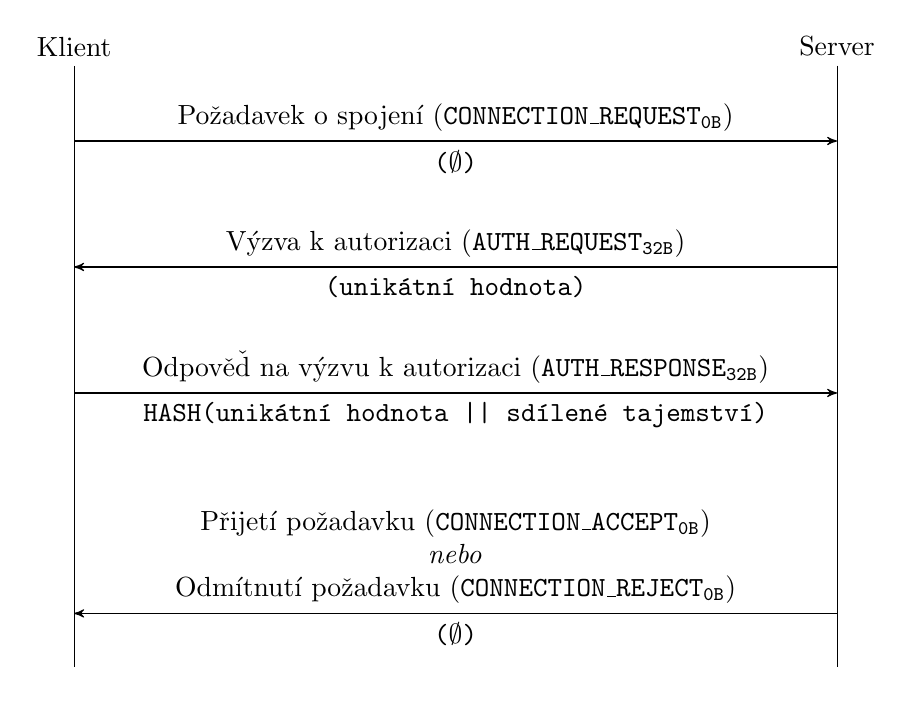
\begin{tikzpicture}[node distance=0.7\textwidth,auto,>=stealth']
    \node[] (Server) {Server};
    \node[left = of Server] (Klient) {Klient};
    \node[below of=Server, node distance=8cm] (server_ground) {};
    \node[below of=Klient, node distance=8cm] (client_ground) {};
    %
    \draw (Klient) -- (client_ground);
    \draw (Server) -- (server_ground);
    \draw[->] ($(Klient)!0.15!(client_ground)$) --
		node[above,scale=1,midway]{Požadavek o spojení (\texttt{CONNECTION\_REQUEST}$_{\texttt{0B}}$)}
		node[below,scale=1,midway]{\texttt{($\emptyset$)}}
	      ($(Server)!0.15!(server_ground)$);
    
    \draw[<-] ($(Klient)!0.35!(client_ground)$) --
		node[above,scale=1,midway]{Výzva k autorizaci (\texttt{AUTH\_REQUEST}$_{\texttt{32B}}$)}
		node[below,scale=1,midway]{\texttt{(unikátní hodnota)}}
	      ($(Server)!0.35!(server_ground)$);
    
    \draw[->] ($(Klient)!0.55!(client_ground)$) --
		node[above,scale=1,midway]{Odpověď na výzvu k autorizaci (\texttt{AUTH\_RESPONSE}$_{\texttt{32B}}$)} 
		node[below,scale=1,midway]{\texttt{HASH(unikátní hodnota || sdílené tajemství)}} 
	      ($(Server)!0.55!(server_ground)$);
    
    \draw[<-] ($(Klient)!0.90!(client_ground)$) --
		node[above,scale=1,align=center]{Přijetí požadavku (\texttt{CONNECTION\_ACCEPT}$_{\texttt{0B}}$)\\ \textit{nebo}\\ Odmítnutí požadavku (\texttt{CONNECTION\_REJECT}$_{\texttt{0B}}$)}
		node[below,scale=1,midway]{\texttt{($\emptyset$)}}
	      ($(Server)!0.90!(server_ground)$);
    
\end{tikzpicture}
\caption{Sekvenční diagram autentizace klienta pomocí protokolu \textit{výzva-odpověď}}
\label{diag:seq-icmp}
\end{figure}
























\chapter{Implementace}
\label{chapter:implementace}

Po návrhu struktury softwarového řešení této diplomové práce následuje samotná implementace. Tato kapitola proto popisuje implementaci řídící části software a jednotlivých \textit{pluginů} pro vytvoření síťového tunelu.


\section{Řídící část softwarového řešení}

Hlavní část programu má na starosti nastartování virtuálního síťového řešení (a v konečné fázi jeho korektní uzavření), kontrolu a přípravu prostředí pro jednotlivé pluginy a umožnění distribuce práce mezi jednotlivými pluginy (a jejich případnými kombinacemi). Dále zahrnuje pomocné části kódu, společné pro všechny pluginy (například nakládání se sdíleným tajemstvím pro autentizaci).

Software vykonává celou řadu nízkoúrovňových operací a značně zasahuje do běhu operačního systému (vytváření nových síťových rozhraní). Z těchto důvodů je nutné software spouštět s oprávněním uživatele \texttt{root}.

\subsection{Požadavky na prostředí}

Pro správnou funkci pluginu pro tunelování pomocí protokolu \texttt{SCTP} je nutná podpora tohoto protokolu v rámci jazyka C. Například pro překladač \texttt{gcc} ji lze zapnout přepínačem \texttt{-lsctp}.

Generování pseudonáhodných dat a výpočet zvolené hashovací funkce je závislé na podpoře knihovny \texttt{OpenSSL} (funkce \texttt{RAND\_bytes} a \texttt{SHA256}). Pro překladač \texttt{gcc} ji lze zapnout přepínačem \texttt{-lssl} nebo případně \texttt{-lcrypto}.

K zajištění flexibility více souběžně pracujících komunikačních pluginů je každému pluginu vytvořeno samostatné pracovní vlákno. Pro práci s vlákny byla zvolena knihovna \texttt{OpenMP}, pro překladač \texttt{gcc} ji lze zapnout přepínačem \texttt{-fopenmp}. Knihovna \texttt{OpenMP} byla sice primárně určena pro datový paralelismus na úrovni cyklů, ale od verze \texttt{3.0} (současná verze \texttt{4.5}) podporuje rovněž funkční paralelismus pomocí direktivy \texttt{task}. Navíc nabízí dobře čitelný zápis a je běžně používanou knihovnou pro paralelizaci, jak zachycuje ukázka kódů \ref{code:mux-start}.

Hlavní část programu rovněž naslouchá na systémové signály typu \texttt{SIGINT} a \texttt{SIGTERM}, díky čemuž je schopna správně ukončit komunikaci, zavřít otevřené sokety a zrušit virtuální rozhraní, pokud se uživatel rozhodne aplikaci ukončit například pomocí \texttt{Ctrl+C}.

    \begin{figure}[h]
	\begin{lstlisting}[caption=Výňatek souboru \texttt{src/mux.c} znázorňující jednoduchost užití knihovny \texttt{OpenMP} pro správu vláken pluginů,language=c,frame=single,numbers=left]
plugin plugins[] = {  [...] };

void muxStart(uint32_t endpoint, bool serverMode)
{
    #pragma omp parallel num_threads(PLUGIN_COUNT)
    #pragma omp single nowait
    for (int i = 0; i < PLUGIN_COUNT; ++i) {
	#pragma omp task
	plugins[i].start(endpoint, serverMode);
    }
}
      \end{lstlisting}
      \label{code:mux-start}
    \end{figure}
    
Systém spuštění \texttt{PLUGIN\_COUNT} vláken nejprve operačnímu systému sdělí, že následující kód je třeba spustit v \texttt{PLUGIN\_COUNT} pomocí direktivy nařádku 5 -- \texttt{nun\_threads()}, která zajistí spuštění kýženého počtu vláken i přestože neodpovídá dostupným prostředkům (počtu dostupných fyzických jader procesoru). Následující direktiva na řádku 6 (\texttt{single nowait}) zajistí, že smyčka na řádcích 7-10 bude vykonána pouze jedním vláknem a následně se provede spuštění požadovaného počtu pluginů, každý ve vlastním vlákně -- pomocí direktivy \texttt{task}.


\section{Plugin pro \texttt{ICMP} tunelování}

Tunelování dat pomocí \texttt{ICMP} je technicky možné díky zprávám typu \texttt{0} a \texttt{8} (\texttt{echo reply}, resp. \texttt{echo request}), pro které je specifikována proměnlivá délka zpráv. Zprávy těchto typů jsou používány zejména nástrojem \texttt{ping} -- například pro zjištění dostupnosti cíle, nebo pro informace o latenci spojení. Zdrojová stanice vyšle na cílovou stanici zprávu typu \texttt{echo request} a cílová stanice odpoví zprávou \texttt{echo reply}. Toto chování je zajištěno v~\cite[RFC1122]{rfc1122}. Strukturu zmíněných \texttt{echo} \texttt{ICMP} zpráv znázorňuje následující diagram \ref{diag:icmp-packet}.


    \begin{figure}[h]
    \centering
	\begin{bytefield}[bitwidth=1em]{32}
	    \bitheader{0,7,8,15,16,31}
	    \\
	    \bitbox{8}{Typ = \texttt{0} (resp. \texttt{8})} & \bitbox{8}{Kód = \texttt{0}} & \bitbox{16}{Kontrolní součet hlavičky}
	    \\
	    \bitbox{16}{Identifikátor} & \bitbox{16}{Sekvenční číslo}
	    \\
	    \wordbox{2}{Data}
	\end{bytefield}
	\caption{Diagram \texttt{ICMP} zprávy typu \texttt{echo request} (resp. \texttt{echo reply})}
	\label{diag:icmp-packet}
    \end{figure}
    
    Protože \texttt{ICMP} pakety \texttt{echo reply}, (resp. \texttt{echo request}) na rozdíl od \texttt{UDP} a \texttt{TCP} paketů nenesou informaci o zdrojovém/cílovém portu, jsou pro sdružování souvisejících zpráv použity hodnoty \textit{identifikátor} a \textit{sekvenční číslo}. Dle \cite[RFC 792]{rfc792} a \cite[RFC 3022]{rfc3022} mohou síťové prvky, jako například \texttt{NAT}, pro rozpoznání souvisejících zpráv tyto hodnoty používat. Specifikace se však nezmiňuje o délce platnosti \textit{identifikátoru}. Díky tomu je možno udržovat obousměrnou komunikaci, i pokud je jeden z účastníků omezen \texttt{NAT}, protože je možné klientovi \uv{za NATem} zaslat více paketů se shodnými hodnotami \textit{sekvenční číslo} a \textit{identifikátor}. Na základě hodnoty \textit{identifikátor} je identifikována i žádost klienta o připojení a následná odpověď na výzvu serveru.
    
    Systém, který dodržuje \cite[RFC1122]{rfc1122} se však bude snažit na příchozí \texttt{ICMP} \textit{echo request} pakety reagovat. Toto chování je pro správnou funkci tunelu nežádoucí. V linuxových distribucích je možné povolit ignorování příchozích zpráv \texttt{ICMP echo} změnou souboru \texttt{/proc/sys/net/ipv4/icmp\_echo\_ignore\_all}.
    
    Aby obě strany tunelu byly schopny identifikovat tok dat tunelu a rozeznat takové zprávy od jiných \texttt{ICMP} zpráv, je nutné \uv{tunelové} \texttt{ICMP} zprávy označit. Právě proto začíná každá taková \texttt{ICMP} zpráva stejnou sekvencí čtyř bajtů, která označuje \texttt{ICMP} zprávy, nesoucí data síťového tunelu. Komunikující protějšky kontrolují zdrojovou \texttt{IP} adresu označených \texttt{ICMP} zpráv, aby nebylo triviálně možné injektovat komunikaci do tunelu. Těchto dodatečných pět bajtů je potřebných pro správnou funkci tunelu a předávání servisních zpráv. Umístění těchto informací v \texttt{ICMP} paketu je vyznačeno na diagramu \ref{diag:icmp-packet-tunel}.
    
    \begin{figure}[h]
    \centering
	\begin{bytefield}[bitwidth=1em]{32}
	    \bitheader{0,7,8,15,16,31}
	    \\
	    \bitbox{8}{Typ = \texttt{0} (resp. \texttt{8})} & \bitbox{8}{Kód = \texttt{0}} & \bitbox{16}{Kontrolní součet hlavičky}
	    \\
	    \bitbox{16}{Identifikátor} & \bitbox{16}{Sekvenční číslo}
	    \\
	    \colorbitbox[ltrb]{lightyellow}{32}{Značka zprávy nesoucí data tunelu}
	    \\
	    \colorbitbox[ltrb]{lightyellow}{8}{Typ zprávy} & \bitbox[lr]{24}{}
	    \\
	    \bitbox[lr]{32}{Data tunelu}
	    \\
	    \bitbox[lbr]{32}{}
	\end{bytefield}
	\caption{Diagram \texttt{ICMP} zprávy typu \texttt{echo request} (resp. \texttt{echo reply}) s vyznačenou hlavičkou dat tunelu}
	\label{diag:icmp-packet-tunel}
    \end{figure}
    
    Značku zpráv tunelu má uživatel možnost změnit při kompilaci programu. Výchozí značkou je sekvence bajtů \verb|0x63 0x76 0x75 0x74|, tedy \texttt{CVUT}.
        
\subsection{Popis jednotlivých typů \texttt{ICMP} zpráv}
\label{subsec:icmp-msg-types}
    
    Typ zprávy označuje jeden z typů, zachycených v ukázce kódu \ref{code:icmp-types}:
        
    \begin{figure}[h]
	\begin{lstlisting}[caption=Výňatek souboru \texttt{plugins/icmp/packet.h} definující typy \texttt{ICMP} zpráv,language=c,frame=single,numbers=left]
typedef enum ICMP_PACKET_TYPE
{
	ICMP_CONNECTION_REQUEST,
	ICMP_AUTH_CHALLENGE,
	ICMP_AUTH_RESPONSE,
	ICMP_CONNECTION_ACCEPT,
	ICMP_CONNECTION_REJECT,
	ICMP_NATPACKET,
	ICMP_KEEPALIVE,
	ICMP_DATA
} ICMP_PACKET_TYPE;
      \end{lstlisting}
      \label{code:icmp-types}
    \end{figure}
    
    Zprávy typu \texttt{CONNECTION\_REQUEST}, \texttt{AUTH\_CHALLENGE}, \texttt{AUTH\_RESPONSE},\\ \texttt{CONNECTION\_ACCEPT}, \texttt{CONNECTION\_REJECT} a \texttt{DATA} jsou implementovány přesně dle specifikace \ref{subsec:msg-types} \textit{Popis základních servisních zpráv}.
    
    \paragraph{} Plugin navíc implementuje zprávu typu \texttt{NATPACKET}:
    
  
  \paragraph{\texttt{NATPACKET}}
    Tyto zprávy odesílá klient a přijímá server. Pokud by klientovi dorazila zpráva tohoto typu, bude ignorována. Server zprávu přijme a poznamená si \textit{identifikátor} a \textit{sekvenční číslo} \texttt{ICMP} zprávy. Tyto údaje následně server použije při odesílání zpráv klientovi. Jedná se o techniku překonání překážek, které způsobuje \texttt{NAT}.
    
  
    
    Situace, kdy se klient připojuje k volnému server je zachycena na diagramu \ref{diag:seq-icmp}.
    

\begin{figure}[h]
 \centering

  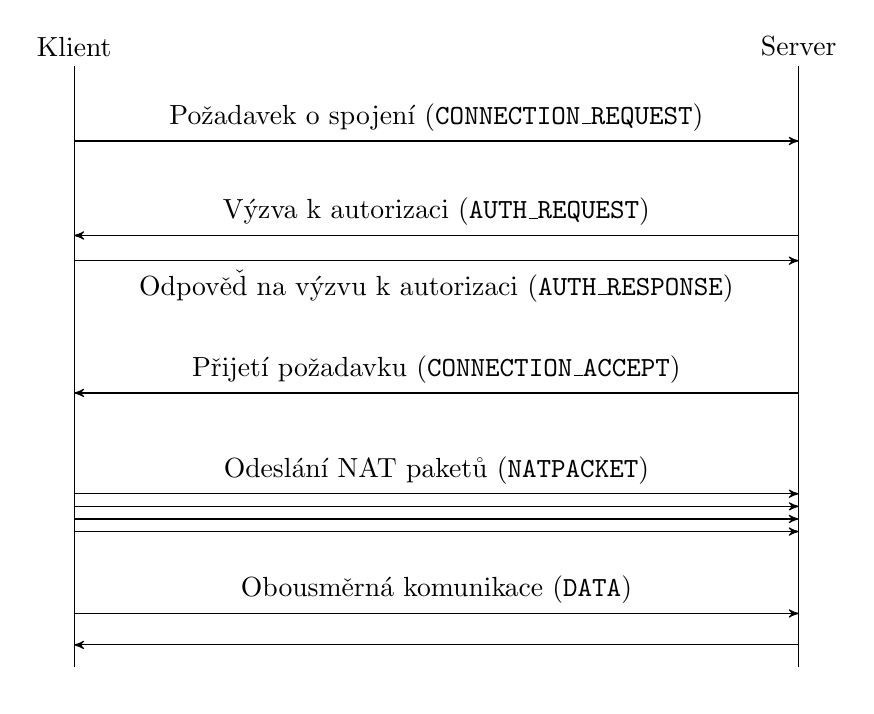
\begin{tikzpicture}[node distance=8cm,auto,>=stealth']
    \node[] (Server) {Server};
    \node[left = of Server] (Klient) {Klient};
    \node[below of=Server, node distance=8cm] (server_ground) {};
    \node[below of=Klient, node distance=8cm] (client_ground) {};
    %
    \draw (Klient) -- (client_ground);
    \draw (Server) -- (server_ground);
    \draw[->] ($(Klient)!0.15!(client_ground)$) -- node[above,scale=1,midway]{Požadavek o spojení (\texttt{CONNECTION\_REQUEST})} ($(Server)!0.15!(server_ground)$);
    
    \draw[<-] ($(Klient)!0.30!(client_ground)$) -- node[above,scale=1,midway]{Výzva k autorizaci (\texttt{AUTH\_REQUEST})} ($(Server)!0.30!(server_ground)$);
    \draw[->] ($(Klient)!0.34!(client_ground)$) -- node[below,scale=1,midway]{Odpověď na výzvu k autorizaci (\texttt{AUTH\_RESPONSE})} ($(Server)!0.34!(server_ground)$);
    
    \draw[<-] ($(Klient)!0.55!(client_ground)$) -- node[above,scale=1,midway]{Přijetí požadavku (\texttt{CONNECTION\_ACCEPT})} ($(Server)!0.55!(server_ground)$);
    
    \draw[->] ($(Klient)!0.71!(client_ground)$) -- node[above,scale=1,midway]{Odeslání \uv{NAT} paketů (\texttt{NATPACKET})}($(Server)!0.71!(server_ground)$);
    \draw[->] ($(Klient)!0.73!(client_ground)$) -- 						 ($(Server)!0.73!(server_ground)$);
    \draw[->] ($(Klient)!0.75!(client_ground)$) -- 						 ($(Server)!0.75!(server_ground)$);
    \draw[->] ($(Klient)!0.77!(client_ground)$) -- 						 ($(Server)!0.77!(server_ground)$);
   
    \draw[->] ($(Klient)!0.90!(client_ground)$) -- node[above,scale=1,midway]{Obousměrná komunikace (\texttt{DATA})} ($(Server)!0.90!(server_ground)$);
    \draw[<-] ($(Klient)!0.95!(client_ground)$) -- 						 ($(Server)!0.95!(server_ground)$);
\end{tikzpicture}
\caption{Sekvenční diagram úspěšného navázání \texttt{ICMP} tunelu}
\label{diag:seq-icmp}
\end{figure}

    
    
    Celková velikost paketu nesoucího zprávu je standardně nastavena na 1500 bajtů -- jedná se o \texttt{MTU} technologie \textit{Ethernet}. To zahrnuje \texttt{IP} hlavičku (20 bajtů), \texttt{ICMP} hlavičku (8 bajtů) a hlavičku zpráv tunelu (5 bajtů). Pro přenášená data je tedy k dispozici až 1467 zbylých bajtů v jedné zprávě. Režie přenosu dat tunelem tvoří 21 bajtů. Vytvářené pakety se drží standardní hodnoty \texttt{MTU} aby bylo (pokud možno) zamezeno fragmentaci. Diagram paketu se všemi hlavičkami je znázorněn na obrázku \ref{diag:icmp-packet-all-headers}.
    
    \begin{figure}[h!]
    \centering
	\begin{bytefield}[bitwidth=1em]{32}
	    \bitheader{0,7,8,15,16,23,24,31}
	    \\
	    \colorwordbox[ltrb]{lightgreen}{5}{IP hlavička (20 bajtů)}
	    \\
	    \colorwordbox[ltrb]{lightcyan}{2}{ICMP hlavička (8 bajtů)}
	    \\
	    \colorwordbox[ltr]{lightyellow}{1}{Hlavička tunelu (5 bajtů)}
	    \\
	    \colorbitbox[lbr]{lightyellow}{8}{} & \bitbox[ltr]{24}{}
	    \\
	    \wordbox[lr]{1}{Data tunelu (až 1467 bajtů)}
	    \\
	    \wordbox[lrb]{1}{}
	\end{bytefield}
	\caption{Diagram paketu včetně rozložení \texttt{ICMP} zprávy tunelu a hlaviček}
	\label{diag:icmp-packet-all-headers}
    \end{figure}
    
    
    
    
    \clearpage
\section{Plugin pro \texttt{UDP} tunelování}
    
    Tunelování dat skrze \texttt{UDP} tunel je primárním principem technologie \textit{OpenVPN}\footnote{\textit{OpenVPN} samozřejmě podporuje i \texttt{TCP} tunelování}. Jedná se o jednoduchý způsob tunelování dat sítí, kdy jsou data tunelu zapouzdřena do \texttt{UDP} datagramů. Protokol \texttt{UDP} nezajišťuje doručení zpráv v původním pořadí a neobsahuje ani mechanismy pro detekci ztracených nebo duplicitních zpráv. Tato zodpovědnost je ponechána na protokolech vyšších vrstev. Strukturu \texttt{UDP} datagramu znázorňuje diagram \ref{diag:udp-packet}.

    \begin{figure}[h]
    \centering
	\begin{bytefield}[bitwidth=.95em]{32}
	    \bitheader{0,7,8,15,16,23,24,31}
	    \\
	    \colorwordbox[ltrb]{lightgreen}{5}{IP hlavička (20 bajtů)}
	    \\
	      \begin{rightwordgroup}{8 bajtů\\ \texttt{UDP} hlavička}
	    \colorbitbox[ltrb]{lightcyan}{16}{Zdrojový port} & \colorbitbox[ltrb]{lightcyan}{16}{Cílový port}
	    \\
	    \colorbitbox[ltrb]{lightcyan}{16}{Délka} & \colorbitbox[ltrb]{lightcyan}{16}{Kontrolní součet} 
	      \end{rightwordgroup}
	    \\
	    \colorwordbox[ltr]{lightyellow}{1}{Hlavička tunelu (5 bajtů)}
	    \\
	    \colorbitbox[lbr]{lightyellow}{8}{} & \bitbox[ltr]{24}{}
	    \\
	    \wordbox[lr]{1}{Data tunelu}
	    \\
	    \wordbox[lrb]{1}{}
	\end{bytefield}
	\caption{Diagram paketu obsahující \texttt{UDP} datagram s daty tunelu}
	\label{diag:udp-packet}
    \end{figure}

Rozdílem oproti tunelování pomocí \texttt{ICMP} je volba portu pro komunikaci. Volbu portu závisí na předpokládané výjimce na firewallu \textit{captive portálu}. Mezi běžné aplikace protokolu \texttt{UDP} patří zejména:

\begin{itemize}
 \item \textit{Domain Name System}, protokol pro překlad doménových jmen, port \texttt{53},
 \item \textit{Network Time Protocol}, protokol pro synchronizaci času, port \texttt{123},
 \item \textit{OpenVPN}, SW pro síťové tunely, port \texttt{1194},
 \item \textit{Session Initiation Protocol}, protokol pro přenos signalizace, port \texttt{5060}
\end{itemize}

Výše zmíněné služby jsou široce rozšířené a je tudíž možné, že pro ně na firewallu \textit{captive portálu} bude existovat výjimka. Například \texttt{IP} telefony typicky nejsou schopny se ověřovat \textit{captive portálu} a právě proto by pro takové zařízení mohla existovat výjimka ve firewallu. Má proto smysl provozovat \texttt{UDP} tunel na takovém portu -- tedy za účelem zvýšení šance nalezení bezpečnostních nedostatků firewallu \textit{captive portálu}. Z výčtu jsem záměrně vynechal některé známé aplikace protokolu \texttt{UDP}, jako například \texttt{DHCP} -- protože má silně lokální charakter a je velmi nepravděpodobné, že by neautentizovaným klientům bylo povoleno komunikovat s \texttt{DHCP} serverem napříč Internetem. Protokol \texttt{DNS} rovněž není vhodným kandidátem, protože pro \texttt{DNS} je v rámci této práce implementována sofistikovanější metoda tunelování dat, blíže popsaná v podkapitole \ref{sec:dns-tunnel} \textit{Plugin pro \texttt{DNS} tunelování}.

Vhodnými kandidáty jsou tedy porty \texttt{123} (\texttt{NTP}) a \texttt{5060} (\texttt{SIP}). Službu \mbox{\textit{OpenVPN}}, která do jisté míry plní podobný účel, lze pohodlně provozovat bok po boku softwarového řešení této diplomové práce. Není proto důvodu zbytečně okupovat výchozí port jiného software.
    
    \subsection{Popis jednotlivých typů \texttt{UDP} zpráv}
        
    Typ zprávy označuje jeden z typů, zachycených v ukázce kódu \ref{code:udp-types}:
        
    \begin{figure}[h]
	\begin{lstlisting}[caption=Výňatek souboru \texttt{plugins/udp/packet.h} definující typy \texttt{UDP} zpráv,language=c,frame=single,numbers=left]
typedef enum UDP_PACKET_TYPE
{
	UDP_CONNECTION_REQUEST,
	UDP_AUTH_CHALLENGE,
	UDP_AUTH_RESPONSE,
	UDP_CONNECTION_ACCEPT,
	UDP_CONNECTION_REJECT,
	UDP_KEEPALIVE,
	UDP_DATA
} UDP_PACKET_TYPE;
      \end{lstlisting}
      \label{code:udp-types}
    \end{figure}

    Z výňatku kódu je patrná analogie s výčtem zpráv \ref{subsec:icmp-msg-types} z podkapitoly \textit{Plugin pro \texttt{ICMP} tunelování}. Jediným rozdílem oproti dříve popsaným typům zpráv je absence zpráv typu \texttt{NATPACKET}, protože protistrana (server) je schopen s klientem za \texttt{NAT} komunikovat díky překladu portů přímo. Klíčové jsou tím pádem \texttt{KEEPALIVE} zprávy, které slouží zejména k přesvědčení \texttt{NAT} zařízení o tom, že komunikace ještě neustala. Díky tomu může server komunikovat s klientem i skrze \texttt{NAT}.
    
    Protože se však význam ostatních zpráv typu \texttt{CONNECTION\_REQUEST}, \texttt{AUTH\_CHALLENGE}, \texttt{AUTH\_RESPONSE},\\ \texttt{CONNECTION\_ACCEPT}, \texttt{CONNECTION\_REJECT} a \texttt{DATA} nijak nemění oproti specifikaci \ref{subsec:msg-types} \textit{Popis základních servisních zpráv}, je jejich opětovný popis vynechán ve prospěch odkazu na původní specifikaci.
     Zprávy 

    Velmi podobný je také sekvenční diagram \ref{diag:seq-udp-tcp} komunikace klienta a serveru při pokusu o navázání spojení. V diagramu se nadále nevyskytují zprávy typu \texttt{NATPACKET}.
    
\begin{figure}[h]
 \centering

  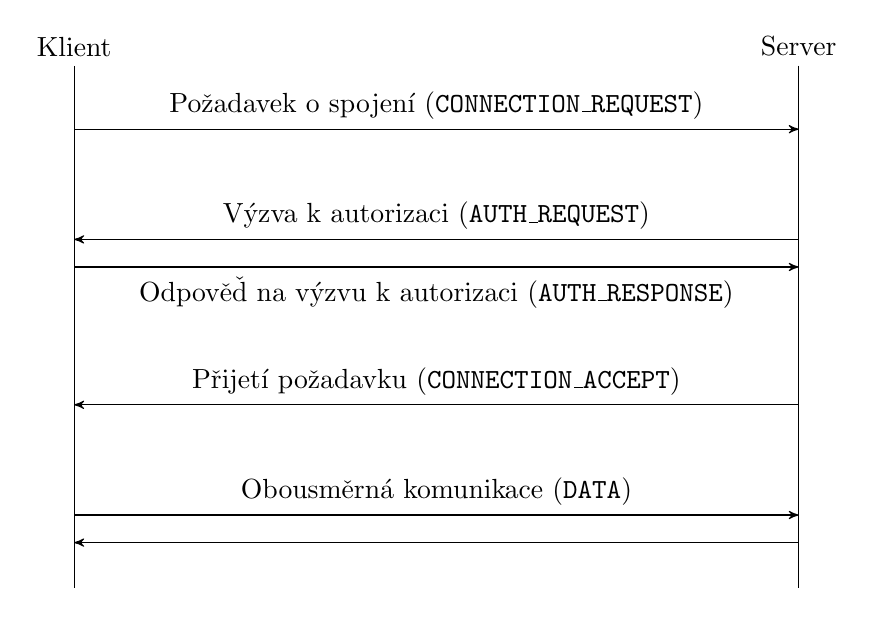
\begin{tikzpicture}[node distance=8cm,auto,>=stealth']
    \node[] (Server) {Server};
    \node[left = of Server] (Klient) {Klient};
    \node[below of=Server, node distance=7cm] (server_ground) {};
    \node[below of=Klient, node distance=7cm] (client_ground) {};
    %
    \draw (Klient) -- (client_ground);
    \draw (Server) -- (server_ground);
    \draw[->] ($(Klient)!0.15!(client_ground)$) -- node[above,scale=1,midway]{Požadavek o spojení (\texttt{CONNECTION\_REQUEST})} ($(Server)!0.15!(server_ground)$);
    
    \draw[<-] ($(Klient)!0.35!(client_ground)$) -- node[above,scale=1,midway]{Výzva k autorizaci (\texttt{AUTH\_REQUEST})} ($(Server)!0.35!(server_ground)$);
    \draw[->] ($(Klient)!0.40!(client_ground)$) -- node[below,scale=1,midway]{Odpověď na výzvu k autorizaci (\texttt{AUTH\_RESPONSE})} ($(Server)!0.40!(server_ground)$);
    
    \draw[<-] ($(Klient)!0.65!(client_ground)$) -- node[above,scale=1,midway]{Přijetí požadavku (\texttt{CONNECTION\_ACCEPT})} ($(Server)!0.65!(server_ground)$);
    
  
    \draw[->] ($(Klient)!0.85!(client_ground)$) -- node[above,scale=1,midway]{Obousměrná komunikace (\texttt{DATA})} ($(Server)!0.85!(server_ground)$);
    \draw[<-] ($(Klient)!0.90!(client_ground)$) -- 						 ($(Server)!0.90!(server_ground)$);
\end{tikzpicture}
\caption{Sekvenční diagram úspěšného navázání \texttt{UDP}/\texttt{TCP} tunelu}
\label{diag:seq-udp-tcp}
\end{figure}


\section{Plugin pro \texttt{TCP} tunelování}

    Protokol \texttt{TCP} je stěžejním členem transportní vrstvy ISO/OSI modelu. Poskytuje spolehlivý přenos dat, garantuje doručení dat ve stejném pořadí v jakém byly odeslány a detekci chyb při přenosu. Díky těmto vlastnostem je velice vhodný pro široké spektrum aplikací -- na moderním Internetu se uživatelé nevědomky setkávají s \texttt{TCP} na každém kroku. Mezi nejrozšířenější aplikace \texttt{TCP} patří zejména protokol \texttt{HTTP}, protokoly pro přenos elektronické pošty (\texttt{IMAP}, \texttt{POP3}, \texttt{SMTP}) a další (\texttt{SSH}, \texttt{FTP}, \texttt{telnet}, \ldots).
    
    Garance doručení, pořadí a detekce chyb s sebou přináší i některé negativní vlastnosti protokolu \texttt{TCP}. Pro aplikace, které vyžadují minimální latenci a rychlou komunikaci, není \texttt{TCP} vhodnou volbou. Zahájení \texttt{TCP} komunikace a případné opakované odesílání dat při ztrátě paketů nejsou ideální zejména pro aplikace v oblasti telefonie nebo živého přenosu obrazu a zvuku. Počítačové hry umožňující hru více hráčů po Internetu mohou rovněž vyžadovat co nejrychlejší provoz s minimální latencí a současně dokáží správně fungovat i při nedoručení části dat.
    
    V takových případech je lepší zvolit jiný, jednodušší protokol transportní vrstvy (typicky \texttt{UDP}). Stejně k problému přistupují i autoři software \textit{OpenVPN}, které primárně podporuje vytváření síťových tunelů pomocí \texttt{UDP}, ale je možné použít i \texttt{TCP}. To však není doporučeno a mělo by být používáno pouze pokud není možné spojení navázat pomocí \texttt{UDP}.
    
    \subsection{Potíže s \texttt{TCP} jako prostředkem pro tunelování}
    \label{subsec:tcp-tunnel-issues}
    
    Jedním z důvodů nevhodnosti \texttt{TCP} jako technologie pro tunelování síťového provozu je fakt, že ne všechen tunelovaný provoz vyžaduje vlastnosti, které \texttt{TCP} nabízí. Implementace \texttt{TCP} obsahuje adaptivní mechanismy pro řízení zatížení linky tak, aby nedošlo k přetížení linky, popsané v \cite[RFC 2001]{rfc2001}. Klíčovým prvkem mechanismu je \textbf{exponenciální} zvyšování délky čekání před opakovaným vysláním nedoručeného segmentu dat. Takové chování však není žádoucí například při \texttt{TCP} komunikaci skrze \texttt{TCP} tunel. Pokud dojde ke ztrátě dat na \texttt{TCP} spojení tunelu, \texttt{TCP} dle implementace zvýší délku čekání před dalším opakovaným vysláním a připraví nedoručená data k opakovanému odeslání. Během této doby dochází k zablokování provozu tunelového spojení a \texttt{TCP} spojení aplikace komunikující skrze tunel nedostane včasné potvrzení protistrany -- a rovněž dojde k zvýšení délky čekání před opakovaným vysláním data, která následně budou skrze tunel odeslána.
    
    Pokud \texttt{TCP} spojení využívající tunel doposud nezvyšovalo délky vyčkávání, dojde k několika zvýšením a k zařazení několika opakovaných odeslání dat zatímco \texttt{TCP} spojení zajišťující tunel je stále zablokované. Každý pokus o opakované vyslání dat skrze tunel problém zhoršuje. Výsledkem je velmi snadno \uv{zamrzající} spojení napříč tunelem, zapříčiněné mechanismy garantující doručení zpráv a pořadí doručení. Tunelované spojení předpokládá standardní nestabilní linku bez garanci doručení -- v případě \texttt{TCP} tunelu je však opak realitou. Tento důsledek tunelování \texttt{TCP} spojení pomocí \texttt{TCP} tunelu je znám jako \textit{meltdown effect}\cite{tcp-over-tcp}.

    
    \subsection{Implementace \texttt{TCP} tunelu}
    
    Struktura tunelovacího nástroje popsaná v podkapitole \ref{subsec:struktura-sw} \textit{Struktura softwarového řešení} umožňuje při implementaci \textit{pluginů} pro jednotlivé tunelovací mechanismy využít již existující kód. Implementace \textit{pluginu} pro \texttt{TCP} tunelování je proto velmi podobná implementaci \textit{pluginu} pro \texttt{UDP} tunelování.
    
    Rozdíly plynou především z rozdílného pojetí komunikace mezi \texttt{UDP} (samostatné zprávy) a \texttt{TCP} (orientace na samostatná spojení a jednotný proud dat). Oproti \texttt{ICMP} tunelování není klíčová identifikace komunikující protistrany, ale délka jednotlivých zpráv v proudu dat. I přes architekturu \texttt{TCP} založenou na konkrétním spojení (oproti \texttt{UDP} bezstavového soketu) zůstaly zachovány \texttt{KEEPALIVE} zprávy, které jsou užitečné zejména při navazování nového spojení -- fáze autentizace. Protože z principu obcházení \textit{captive portálu} je \textit{plugin} navržen pro obsluhu pouze jednoho spojení, mohlo by docházet k blokování dostupného spojení jinými připojujícími se uzly v Internetu. Server tedy ignoruje \texttt{KEEPALIVE} zprávy až do chvíle, kdy se klient úspěšně autentizuje. Z pohledu serveru je klient před úspěšnou autentizací nedostupný, resp. již není na příjmu (ignorování \texttt{KEEPALIVE} zpráv) a bude odpojen, pokud se úspěšně neověří před vypršením maximální délky bez přijetí \texttt{KEEPALIVE} zprávy.
    
    Sekvenční diagram \ref{diag:seq-udp-tcp} komunikace klienta a serveru při pokusu o navázání spojení je identický s pluginem pro \texttt{UDP} tunelování.
    
    \subsection{Volba portu pro provoz \texttt{TCP} tunelu}
    
    S přihlédnutím k nesmírné popularitě a rozšířenosti protokolu \texttt{TCP} se k maskování tunelového provozu nabízí celá řada \texttt{TCP} portů. Volbou může být port \texttt{80}, resp \texttt{443} (\texttt{HTTP}, resp. \texttt{HTTPS}). S provozem cíleným na tyto porty však \textit{captive portál} zpravidla manipuluje a nelze tak dopředu říci, jaká je šance na úspěšné obejití omezení \textit{captive portálu}. Alternativní volbu představuje port \texttt{3128}, který může mít ve firewallu výjimku za účelem provozu \texttt{HTTP} caching proxy (správce \textit{hotspotu} může takovou službu provozovat za účelem šetření přenesených dat směrem z/do Internetu).
    
    Možnou volbou je i port \texttt{TCP/22}, jehož užití s sebou však ponese nutnost změny portu \texttt{SSH} služby, který na serveru s velkou pravděpodobností je provozován.
    
    Není možné předem s jistotou říci, pro jaký (nebo zda-li vůbec nějaký) port má konkrétní \textit{captive portál} ve firewallu nastavenou výjimku. Volba portu je uživatelsky nastavitelná a záleží tedy na zvážení uživatele software, kolik instancí \texttt{TCP} pluginu pro různé porty hodlá provozovat.
    
    \subsection{Návrh formátu datové zprávy}
    
    Z diagramu návrhu zprávy je dobře patrná výrazně větší režie \texttt{TCP} spojení (32 bajtů hlavičky oproti dosavadním 8 bajtům u \texttt{ICMP} a \texttt{UDP}). Protože \texttt{TCP} přistupuje k přenášeným datům jako k proudu dat, není zaručené, že jednotlivé zprávy budou mít vždy tento formát. Každá zpráva začíná jednobajtovým identifikátorem typu zprávy (servisní a její typ, nebo datová) a je následován velikostí zprávy (2 bajty). Velikost umožňuje specifikovat velikost až zprávy až 65535 bajtů, té by však nemělo být nikdy dosaženo, protože do tunelu data proudí z virtuálního síťového rozhraní, které má standardní \texttt{MTU} 1500 bajtů.
    
    Velikost dat je přenášena ve dvou bajtech -- nižších 8 bitů a vyšších 8 bitů samostatně pomocí maskování původní nezáporné šestnáctibajtové délky dat. Čtení dat z \texttt{TCP} proudu probíhá ve smyčce, která vždy:
    \begin{enumerate}
     \item Přečte jeden bajt (typ zprávy),
     \item Přečte dva bajty a rekonstruuje velikost data,
     \item Provede neblokující čtení dokud nepřečte přesně specifikované množství dat.
    \end{enumerate}
    
    
    
    \begin{figure}[h]
    \centering
	\begin{bytefield}[bitwidth=1em]{32}
	    \bitheader{0,7,8,15,16,23,24,31}
	    \\
	    \colorwordbox[ltrb]{lightgreen}{5}{IP hlavička (20 bajtů)}
	    \\
	    \colorwordbox[ltrb]{lightcyan}{8}{TCP hlavička (32 bajtů)}
	    \\
	    \colorbitbox[ltbr]{lightyellow}{8}{Typ zprávy} & \colorbitbox[ltbr]{lightyellow}{16}{Velikost dat (2 bajty)} & \bitbox[ltr]{8}{}
	    \\
	    \wordbox[lr]{1}{}
	    \\
	    \wordbox[lr]{1}{Data tunelu}
	    \\
	    \wordbox[lrb]{1}{}
	\end{bytefield}
	\caption{Diagram \texttt{TCP} zprávy s vyznačenou hlavičkou dat tunelu, délkou \texttt{TCP} hlavičky a délkou \texttt{IP} hlavičky}
	\label{diag:tcp-packet-tunel}
    \end{figure}
    
    \clearpage
\section{Plugin pro \texttt{SCTP} tunelování}

    \texttt{SCTP} je protokolem transportní vrstvy ISO/OSI modelu, stejně jako protokoly \texttt{TCP} nebo \texttt{UDP}. Přebírá některé volitelné vlastnosti těchto protokolů, například volitelnou obdobu \texttt{TCP} garanci doručení paketů ve správném pořadí, nebo \texttt{UDP} způsob komunikace (oproti \texttt{TCP} proudové komunikaci). Navíc přidává funkce jako multihoming nebo víceproudovou komunikaci v rámci jednoho spojení. Jedná se o \textit{relativně} mladý protokol, definovaný v \cite[RFC 4960]{rfc4960} v roce 2007.
    
    Stejně jako u \texttt{ICMP} je možné, že implementace \textit{captive portálu} nebude pamatovat na jiné protokoly než \texttt{TCP} a \texttt{UDP}. Právě proto je v rámce této práce implementován rovněž tunel pomocí \texttt{SCTP} protokolu. Jeho vlastnosti navíc umožňují efektivněji pracovat se spojením -- zejména oproti \texttt{TCP} tunelu.
    
    \subsection{Víceproudovost}
    
    \texttt{SCTP} umožňuje v rámci jednoho spojení (\textit{asociace}) komunikovat pomocí vícero nezávislých datových proudů. Tato vlastnost nachází praktické využití například v \texttt{IP} telefonii, kdy je možné v rámci jednoho spojení přenášet odděleně signalizaci a samotná hlasová data.
    
    Pro účely této práce je tato vlastnost užitečná, protože kromě čistšího návrhu protokolu, který nemíchá servisní zprávy a data dohromady, tento přístup částečně řeší problém známý jako \textit{head-of-line blocking}. Ten nastává zejména při zablokování datového proudu (například kvůli ztrátě paketu a čekání na opakované odeslání). Proud dat je tedy blokován první zprávou, která nebyla úspěšně doručena. Čekání na další postup brání prostupu jiných dat, zejména servisních zpráv. Oddělené datové proudy pro servisní zprávy a samotná data tunelu tento problém společně s \ref{subsec:sctp-unordered-delivery} doručením v náhodném pořadí řeší problém \textit{head-of-line blocking}.
    
      
\begin{figure}[h]
 \centering

  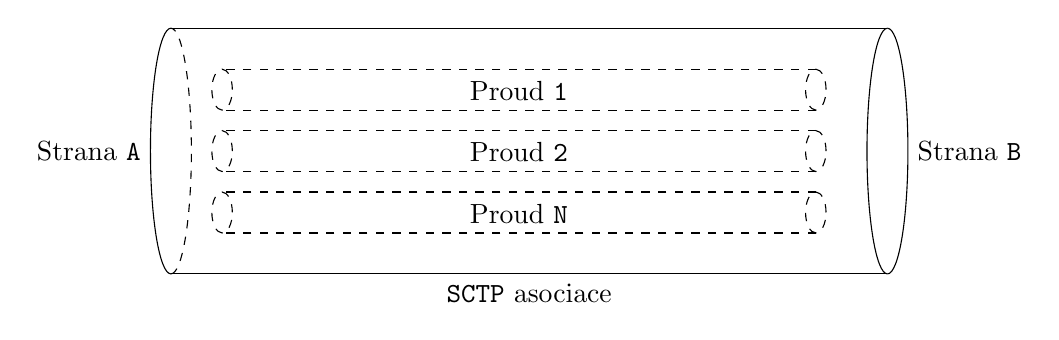
\begin{tikzpicture}[scale=1.3]
\draw (0,-1.2) arc (270:90:0.2 and 1.2);
\draw (0,-1.2) arc (90:270:-0.2 and -1.2) node[right,midway]{Strana \texttt{B}};
\draw (0,-1.2) -- (-7.0,-1.2) node[below,midway]{\texttt{SCTP} asociace};
\draw (-7.0,-1.2) arc (270:90:0.2 and 1.2) node[left,midway]{Strana \texttt{A}};
\draw [dashed] (-7.0,-1.2) arc (90:270:-0.2 and -1.2);
\draw (-7.0,1.2) -- (0,1.2);


\draw [dashed] (-0.7,0.6) ellipse (0.1 and 0.20);
\draw [dashed] (-0.7,0.4) -- node[above]{Proud \texttt{1}} (-6.5,0.4);
\draw [dashed] (-0.7,0.8) -- (-6.5,0.8);
\draw [dashed] (-6.5,0.6) ellipse (0.1 and 0.20);


\draw [dashed] (-0.7,0.0) ellipse (0.1 and 0.20);
\draw [dashed] (-0.7,-0.2) -- node[above]{Proud \texttt{2}} (-6.5,-0.2);
\draw [dashed] (-0.7,0.2) -- (-6.5,0.2);
\draw [dashed] (-6.5,0.0) ellipse (0.1 and 0.20);


\draw [dashed] (-0.7,-0.6) ellipse (0.1 and 0.20);
\draw [dashed] (-0.7,-0.8) -- node[above]{Proud \texttt{N}} (-6.5,-0.8);
\draw [dashed] (-0.7,-0.4) -- (-6.5,-0.4);
\draw [dashed] (-6.5,-0.6) ellipse (0.1 and 0.20);


\end{tikzpicture}
\caption{Vztah proudů spojení a \texttt{SCTP} asociace}
\label{diag:sctp-streams}
\end{figure}
    
    \subsection{Doručení v náhodném pořadí}
    \label{subsec:sctp-unordered-delivery}
    
    Protokol \texttt{SCTP} respektuje hranice zpráv. Díky tomu programátorovi nabízí možnost nevynucovat doručení zpráv ve stejném pořadí, v jakém byly odeslány. Tato vlastnost je pro implementaci tunelu velice vhodná, protože \textit{nevnucuje} garanci pořadí doručení veškerému provozu a deleguje odpovědnost na protokoly vyšších vrstev.
    
    
    
    
  
    \subsection{Popis jednotlivých typů \texttt{SCTP} zpráv}
        
    Díky víceproudovosti transportního protokolu \texttt{SCTP} dochází ke kompletnímu oddělení dat tunelu a servisních zpráv pro řízení tunelu. Jednotlivé servisní zprávy jsou zachyceny v ukázce kódu \ref{code:sctp-types}:
        
    \begin{figure}[h]
	\begin{lstlisting}[caption=Výňatek souboru \texttt{plugins/sctp/packet.h} definující typy \texttt{SCTP} zpráv,language=c,frame=single,numbers=left]
typedef enum SCTP_PACKET_TYPE
{
	SCTP_CONNECTION_REQUEST,
	SCTP_AUTH_CHALLENGE,
	SCTP_AUTH_RESPONSE,
	SCTP_CONNECTION_ACCEPT,
	SCTP_CONNECTION_REJECT,
	SCTP_KEEPALIVE
} SCTP_PACKET_TYPE;
      \end{lstlisting}
      \label{code:sctp-types}
    \end{figure}
    
    Počet typů servisních zpráv je oproti ostatním implementovaným tunelům omezen na nejnutnější minimum. Jsou implementovány přesně dle specifikace popsané v podkapitole \ref{subsec:msg-types} \textit{Popis základních servisních zpráv}. Protože se však význam ostatních zpráv nijak nemění, je jejich opětovný popis vynechán s odkazem na jejich specifikaci v podkapitole \ref{subsec:msg-types}. Lehce odlišný je však sekvenční diagram \ref{diag:seq-udp-tcp} komunikace klienta a serveru při pokusu o navázání spojení. V diagramu se nadále nevyskytují zprávy typu \texttt{DATA}, protože data tunelu jsou přenášena samostatným datovým proudem.
    
    
\begin{figure}[h]
 \centering

  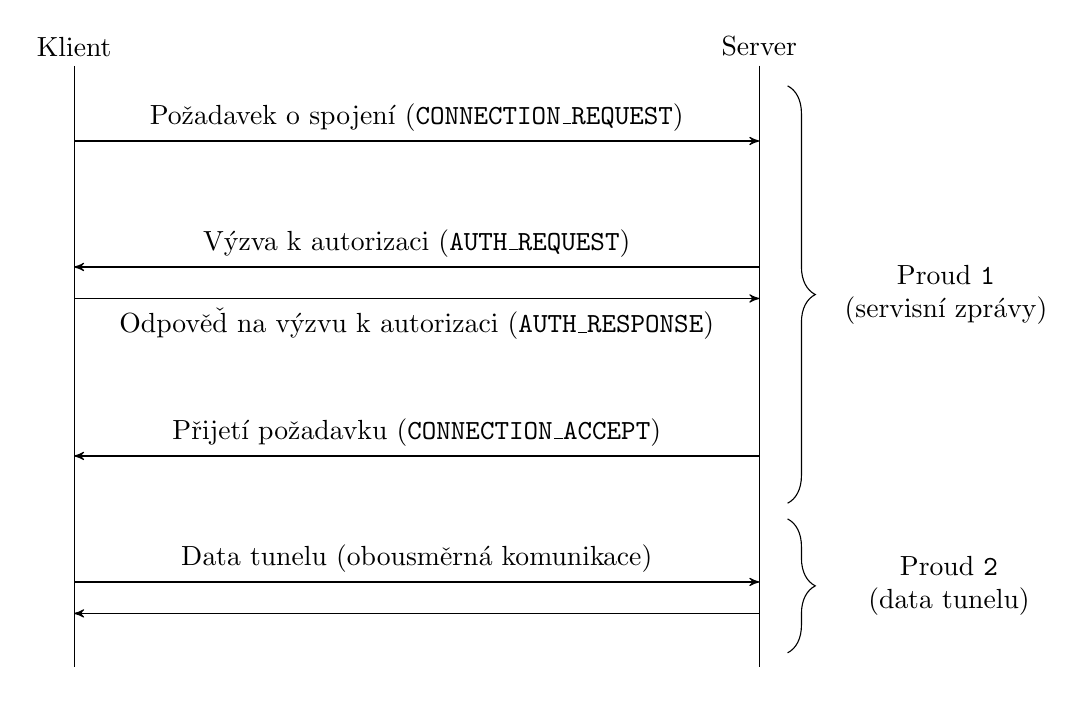
\begin{tikzpicture}[node distance=7.5cm,auto,>=stealth']
    \node[] (Server) {Server};
    \node[left = of Server] (Klient) {Klient};
    \node[below of=Server, node distance=8cm] (server_ground) {};
    \node[below of=Klient, node distance=8cm] (client_ground) {};
    %
    \draw (Klient) -- (client_ground);
    \draw (Server) -- (server_ground);
    \draw[->] ($(Klient)!0.15!(client_ground)$) -- node[above,scale=1,midway]{Požadavek o spojení (\texttt{CONNECTION\_REQUEST})} ($(Server)!0.15!(server_ground)$);
    
    \draw[<-] ($(Klient)!0.35!(client_ground)$) -- node[above,scale=1,midway]{Výzva k autorizaci (\texttt{AUTH\_REQUEST})} ($(Server)!0.35!(server_ground)$);
    \draw[->] ($(Klient)!0.40!(client_ground)$) -- node[below,scale=1,midway]{Odpověď na výzvu k autorizaci (\texttt{AUTH\_RESPONSE})} ($(Server)!0.40!(server_ground)$);
    
    \draw[<-] ($(Klient)!0.65!(client_ground)$) -- node[above,scale=1,midway]{Přijetí požadavku (\texttt{CONNECTION\_ACCEPT})} ($(Server)!0.65!(server_ground)$);
    
  
    \draw[->] ($(Klient)!0.85!(client_ground)$) -- node[above,scale=1,midway]{Data tunelu (obousměrná komunikace)} ($(Server)!0.85!(server_ground)$);
    \draw[<-] ($(Klient)!0.90!(client_ground)$) -- 						 ($(Server)!0.90!(server_ground)$);
    
    \draw [decorate,decoration={brace,amplitude=10pt},xshift=-4pt,yshift=0pt]
(.5,-0.5) -- (.5,-5.8) node [align=center,midway,xshift=0.6cm]{Proud \texttt{1}\\(servisní zprávy)};

\draw [decorate,decoration={brace,amplitude=10pt},xshift=-4pt,yshift=0pt]
 (.5,-6) -- (.5,-7.7) node [align=center,midway,xshift=0.9cm]{Proud \texttt{2}\\(data tunelu)};
    
\end{tikzpicture}
\caption{Sekvenční diagram úspěšného navázání \texttt{SCTP} tunelu}
\label{diag:seq-sctp}
\end{figure}

    
    \subsection{Volba portu pro provoz \texttt{SCTP} tunelu}
    
    Pointou implementace \texttt{SCTP} pluginu je možná nedbalost správce \textit{firewallu}, či nedokonalost \textit{captive portálu}, která neomezuje provoz protokolu \texttt{SCTP}. Uživatel tedy není limitován snahou o maskování provozu tunelu jako jiné legitimní či neblokované činnosti. Nevelká rozšířenost protokolu \texttt{SCTP} však umožňuje obsadit známé \texttt{TCP} porty na \texttt{SCTP} socketech aniž by došlo k narušení jiných bežících služeb. Opět platí, že konkrétní volbu nelze s jistotou předem předpovědět a je tak na zvážení uživatele, jaké výjimky ve firewallu by mohlo daná síť mít.

    \subsection{Návrh formátu datové zprávy}
    
    Protokol \texttt{SCTP} disponuje hlavičkou o velikosti 32 bajtů, velikostně menší, než \texttt{TCP} (38 bajtů), ale větší než \texttt{ICMP} a \texttt{UDP} (8 bajtů). Zato však disponuje možností odeslání několika zpráv (\textit{chunks}) v jednom paketu (což zahrnuje i \texttt{IP} hlavičku) při zachování hranic zpráv. Protože \texttt{SCTP} umožňuje komunikovat pomocí oddělených a nezávislých datových proudů, není pro datové zprávy nutné specifikovat hlavičku dat tunelu, protože všechny servisní zprávy používají vlastní proud. \uv{Střední} velikost hlavičky je tedy vyvážena výhodami protokolu \texttt{SCTP}.
    
    Protistrana tak může data rovnou zapisovat do virtuálního rozhraní a nemusí se zabývat čekáním na více zpráv a jejich následnému skládání (za předpokladu, že díky servisním zprávám již proběhla autentizace).
    
    \begin{figure}[h]
    \centering
	\begin{bytefield}[bitwidth=1em]{32}
	    \bitheader{0,7,8,15,16,23,24,31}
	    \\
	    \colorwordbox[ltrb]{lightgreen}{5}{IP hlavička (20 bajtů)}
	    \\
	    \colorwordbox[ltrb]{lightcyan}{7}{SCTP hlavička (32 bajtů)}
	    \\
	    \wordbox[lr]{1}{}
	    \\
	    \wordbox[lr]{1}{Kusy (\textit{chunks}) dat tunelu}
	    \\
	    \wordbox[lrb]{1}{}
	\end{bytefield}
	\caption{Diagram \texttt{SCTP} zprávy nezávislého datového proudu (tedy bez redundantní hlavičky dat tunelu) a s vyznačenou délkou \texttt{SCTP} hlavičky a délkou \texttt{IP} hlavičky}
	\label{diag:tcp-packet-tunel}
    \end{figure}
    
    \clearpage
    
\section{Plugin pro \texttt{DNS} tunelování}
\label{sec:dns-tunnel}
    
    Protokol \texttt{DNS} je jedním z hlavních pilířů infrastruktury moderního Internetu. Umožňuje překládat doménová jména na \texttt{IP} adresy a poskytovat další související informace o konkrétní doméně, například pro poštovní servery.
    
    Tunelování pomocí \texttt{DNS} staví na odlišném principu, než doposud všechny navržené a implementované pluginy. Největším rozdílem je, že oproti \texttt{TCP}, \texttt{UDP} a \texttt{SCTP} tunelům nespoléhá na navázání spojení se serverem v Internetu, ale podobně jako \texttt{ICMP} se snaží přimět okolní infrastrukturu, aby zprávy předala k cílovému serveru v Internetu a odpověď dopravila zpět. Základním mechanismem \texttt{DNS} tunelování jsou \texttt{DNS} servery, které umí zpracovat rekurzivní \texttt{DNS} požadavky.
    
    \subsection{Principy \texttt{DNS} tunelování}
    
    Základním principem služby \texttt{DNS} je hierarchická struktura \textit{jmenných serverů}\footnote{Pro potřeby této práce je v textu rovněž použito označení \uv{\texttt{DNS} server}}, které jsou schopny odpovídat na \texttt{DNS} dotazy od klientských překladačů (\textit{resolver}). Pokud jmenný server nezná odpověď na dotaz, může
    
    \begin{itemize}
     \item klienta odkázat na jiný jmenný server (nerekurzivní chování),
     \item odpověď sám dohledat dotazem na další jmenné servery a vrátit klientovi (rekurzivní chování).
    \end{itemize}
    
    Pokud jmenný server je ochoten rekurzivně vyhodnocovat dotazy, může klient tento server přimět ke komunikaci s okolním světem. Klient může v tomto případě přesně \textit{nasměrovat} rekurzivní \texttt{DNS} server do části Internetu, kterou klient ovládá (například provozuje svůj vlastní \texttt{DNS} server). V této pozici je tedy klient schopen komunikovat prostřednictvím rekurzivního \texttt{DNS} serveru s jiným svým systémem, dostupným přes síť Internet. Protože klient ovládá cílový \texttt{DNS} server, má tím pádem kontrolu i nad daty, která budou rekurzivním \texttt{DNS} serverem klientovi vrácena jako odpověď na jeho požadavek. Výsledkem je možnost obousměrné komunikace do Internetu pouze prostřednictvím dostupného \texttt{DNS} serveru ochotného zpracovávat rekurzivní dotazy.

    Protože se však jedná o komunikaci skrze prostředníka, je pro \texttt{DNS} tunelování nutné zachovat specifikace \texttt{DNS} protokolu dle \cite[RFC 1035]{rfc1035}. Z toho však plynou nutná omezení pro tunelování síťového provozu -- nemožnost \textit{plně} oboustranné komunikace, protože klientův \texttt{DNS server} v Internetu nemá žádnou možnost, jak dopravit data ke klientovi, pokud nemá žádný klientův \texttt{DNS} dotaz k zodpovězení.
    
    Tento nedostatek lze vyřešit metodou \textit{polling}, kdy se klient serveru opakovaně zprostředkovaně dotazuje, pro případ, že server má data, která je třeba dopravit ke klientovi. Toto řešení s sebou však nese výrazně sníženou prostupnost tunelového spojení. 
    

  \begin{figure}
  \centering
    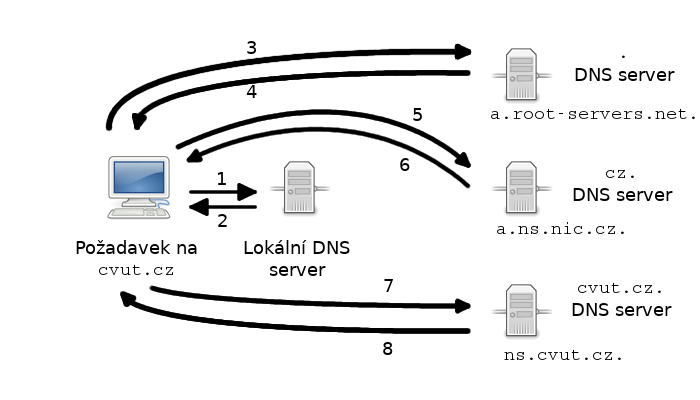
\includegraphics[width=\textwidth]{attachments/dns_iterative.png}
    \caption{Ukázka iterativního (nerekurzivního) \texttt{DNS} dotazu. Klient se \texttt{DNS} serverů dotazuje sám. Buď dostane odpověď, nebo je odkázán na jiný \texttt{DNS} server.}
    \label{pic:dns-iterative}
  \end{figure}
    
  \begin{figure}
  \centering
    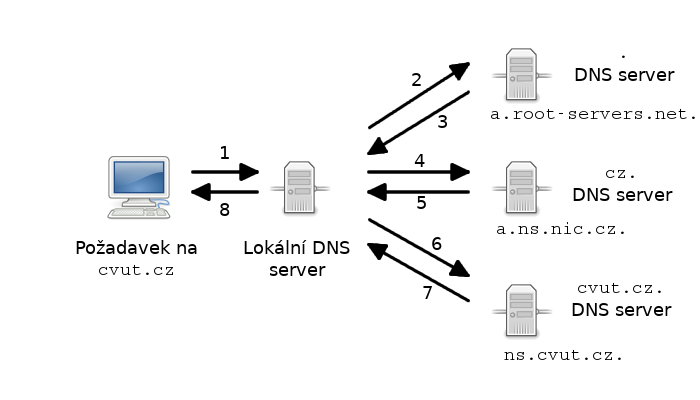
\includegraphics[width=\textwidth]{attachments/dns_recursive.png}
    \caption{Ukázka rekurzivního \texttt{DNS} dotazu. Lokální \texttt{DNS} server prohledá svou \textit{cache} a pokud v ní nenalezne odpověď na klientův dotaz, začne odpověď hledat dotazy na jiné \texttt{DNS} servery.}
    \label{pic:dns-recursive}
  \end{figure}

\clearpage




    
    
    % vysvetlit vysvetlit, neimplementujeme, je to pomale, ale zmerime deset ruznych tunelovacich nastorju, abychom ukazali jak pomale to je .. nam jde o prostupnost, tohle nikoho nezajima + velky traffic nas muze odriznout
    
    


\chapter{Testování}

Doplňte vhodný text.


\begin{conclusion}
	Doplňte závěr.
	
\end{conclusion}

\bibliographystyle{csn690}
\bibliography{literatura}

\appendix

\chapter{Seznam použitých zkratek}
% \printglossaries



%TODO sort a-z
\begin{description}
	\item[DNS] Domain Name System
	\item[ICMP] Internet Control Message Protocol
	\item[XML] Extensible markup language
	\item[ISM] Industrial, Scientific and Medical radio bands
	\item[NAC] Network Access Control -- řízení síťového přístupu
	\item[GSM] Global System for Mobile Communications
	\item[MAC] Media Access Control
	\item[IP] Internet Protocol
	\item[SIP] Session Initiation Protocol
	\item[MITM] Man-in-the-middle
	\item[HTTP] Hypertext Transfer Protocol
	\item[MTU] Maximum transmission unit
	\item[HTTPS] HTTP Secure
	\item[TTL] Time to live
	\item[SOCKS] Socket Secure
	\item[NAT] Network Address Translation
	\item[SSH] Secure Shell
	\item[TCP] Transmission Control Protocol
	\item[UDP] User Datagram Protocol
	\item[RADIUS] Remote Authentication Dial-In User Service
	\item[VLAN] Virtual local area network
	\item[WWW] World wide web
	\item[WPA] Wi-Fi Protected Access
	\item[WISPr] Wireless Internet Service Provider roaming
	\item[VoIP] Voice over IP
	\item[VPN] Virtual private network
\end{description}


% LaTeX notes:

% citace: viz \cite{kobltypo}

% vlna

% \begin{figure}\centering
% 	
\includegraphics[width=0.5\textwidth, angle=30]{cvut-logo-bw}
% 	\caption[Příklad obrázku]{Ukázkový obrázek v~plovoucím prostředí}\label{fig:float}
% \end{figure}

%Může se hodit mít více verzí stejného obrázku, např. pro barevný či černobílý tisk a nebo pro prezentaci.

% label -> (viz obr. \ref{fig:gnuplot-bw}) 

% \subsection{Tabulky}
% 
% Tabulky lze zadávat různě, např. v~prostředí \verb|tabular|, avšak pro jejich vkládání platí to samé, co pro obrázky -- použijte plovoucí prostředí, v~tomto případě \verb|table|. Například tabulka \ref{tab:matematika} byla vložena tímto způsobem.
% 
% \begin{table}\centering
% 	\caption[Příklad tabulky]{Zadávání matematiky}\label{tab:matematika}
% 	\begin{tabular}{|l|l|c|c|}\hline
% 		Typ		& Prostředí		& \LaTeX{}ovská zkratka	& \TeX{}ovská zkratka	\tabularnewline \hline \hline
% 		Text		& \verb|math|		& \verb|\(...\)|	& \verb|$...$|		\tabularnewline \hline
% 		Displayed	& \verb|displaymath|	& \verb|\[...\]|	& \verb|$$...$$|	\tabularnewline \hline
% 	\end{tabular}
% \end{table}


% vkládání URL a podobných informací url{} ze stejnojmenného balíčku. Zajistíte tím jednak odlišení adresy od ostatního textu pomocí jiného písma a také zalamování na konci řádku.
% Chcete-li vkládat odkazy (funkční v~PDF), použijte příkaz \verb|href| z~balíčku \verb|hyperref|.

% % % % % % % % % % % % % % % % % % % % % % % % % % % 

\chapter{Obsah přiloženého CD}


% Vhodným způsobem vizualizujte obsah přiloženého média. Lze použít balíček \verb|dirtree| a vytvořit např. následující výstup (adresáře src a text s~příslušným obsahem jsou \emph{povinné}):
% 
% \begin{figure}
% 	\dirtree{%
% 		.1 readme.txt\DTcomment{stručný popis obsahu CD}.
% 		.1 exe\DTcomment{adresář se spustitelnou formou implementace}.
% 		.1 src.
% 		.2 impl\DTcomment{zdrojové kódy implementace}.
% 		.2 thesis\DTcomment{zdrojová forma práce ve formátu \LaTeX{}}.
% 		.1 text\DTcomment{text práce}.
% 		.2 thesis.pdf\DTcomment{text práce ve formátu PDF}.
% 	}
% \end{figure}


\end{document}
